\documentclass[11pt,a4paper,twoside]{report}
\usepackage[utf8]{inputenc}
\usepackage[T1]{fontenc}
\usepackage[spanish,es-tabla]{babel} % es-tabla para que diga "Tabla" en lugar de "Cuadro"

% Márgenes según manual: Superior, Inferior y Derecho 2.5 cm; Izquierdo 3 cm
\usepackage[top=2.5cm, bottom=2.5cm, left=3cm, right=2.5cm]{geometry}

% Tipo de letra: Times New Roman 11 (mathptmx es la versión libre de LaTeX)
\usepackage{mathptmx} 

% Interlineado 1.5 en el texto general
\usepackage{setspace}
\onehalfspacing

% Configuración de Títulos según manual
\usepackage{titlesec}

% Capítulo: Negrita, tamaño 14
\titleformat{\chapter}[display]
{\normalfont\fontsize{14}{16}\bfseries}
{\chaptertitlename\ \thechapter}{10pt}{\fontsize{14}{16}\bfseries}

% Sección 1.1: Negrita, tamaño 12
\titleformat{\section}
{\normalfont\fontsize{12}{14}\bfseries}
{\thesection}{0.5em}{}

% Sub-sección 1.1.1: Negrita, tamaño 12
\titleformat{\subsection}
{\normalfont\fontsize{12}{14}\bfseries}
{\thesubsection}{0.5em}{}

% Sub-sub-sección 1.1.1.1: Negrita, tamaño 12 
\titleformat{\subsubsection}
{\normalfont\fontsize{12}{14}\bfseries}
{\thesubsubsection}{0.5em}{}

\setcounter{secnumdepth}{2}
\setcounter{tocdepth}{2}

% Redacción del texto general ya es tamaño 11pt normal por \documentclass[11pt]

\usepackage{graphicx}
\usepackage{caption}
% Espacio de 3 líneas después de imágenes y tablas (aprox 3em)
\setlength{\intextsep}{0.5em}

\usepackage{tocbibind} % Para que aparezcan los índices en la tabla de contenidos

\usepackage[utf8]{inputenc} % Soporte para caracteres especiales (acentos, ñ)
\usepackage{booktabs} % Bordes profesionales (\toprule, \midrule, \bottomrule, \addlinespace)
\usepackage{tabularx} % Tablas ajustables al ancho de página (columna tipo X)
\usepackage{array} % Modificadores de alineación en columnas (>{\raggedright\arraybackslash})
\usepackage{ragged2e} % Permite auto-ajuste de texto con guiones dentro de tablas

\begin{document}
	
	% Numeración romana para páginas preliminares
	\pagenumbering{roman}
	\setcounter{page}{1} % La portada es i, pero no se numera visiblemente
	
	% ==========================================
	% PORTADA
	% ==========================================
	\thispagestyle{empty}
	\begin{center}
		
		
\includegraphics[width=0.45\textwidth]{unc.png} \\[0.5cm] % Logo
		
		{\large UNIVERSIDAD NACIONAL DE CÓRDOBA} \\[0.5cm]
		{\large FACULTAD DE CIENCIAS EXACTAS, FÍSICAS Y NATURALES} \\[0.5cm]
		{\large CARRERA INGENIERÍA ELECTRÓNICA} \\[0.5cm]
		
		{\large PROYECTO INTEGRADOR PARA LA OBTENCIÓN DEL TÍTULO DE GRADO INGENIERO ELECTRÓNICO} \\[1.5cm]
		
		{\Large \textbf{“DISEÑO E IMPLEMENTACION DE ETAPA RECEPTORA DE TRANSPONDER CUBESAT VHF-UHF”}} \\[2cm]
		
		\begin{flushleft}
			\textbf{Alumno/s:} \\
			Apellido, Nombre y Apellido, Nombre \\[1cm]
			
			\textbf{Director:} \\
			Dr./Mgr./Esp./Ing. Apellido, Nombre \\[1cm]
			
			\textbf{Co-Director:} \\
			Dr./Mgr./Esp./Ing. Apellido, Nombre \\[1cm]
		\end{flushleft}
		
		\vfill
		{\large Córdoba, República Argentina} \\
		{\large Mes / Año}
	\end{center}
	\clearpage
	
	% ==========================================
	% CONTRATAPA (TRIBUNAL EVALUADOR)
	% ==========================================
	\thispagestyle{empty}
	\begin{center}
		
		
\includegraphics[width=0.45\textwidth]{unc.png} \\[2cm] % Logo
		
		UNIVERSIDAD NACIONAL DE CÓRDOBA \\
		Facultad de Ciencias Exactas, Físicas y Naturales \\
		Escuela de Ingeniería Electrónica
	\end{center}
	\vspace{1cm}
	El Tribunal Evaluador reunido en éste acto y luego de haber aprobado la Solicitud 
	de Aprobación de Tema y efectuado las distintas instancias de correcciones del Informe 
	del Proyecto Integrador para la obtención del Título de Grado “Ingeniero Electrónico” y 
	cumpliendo con el Reglamento correspondiente, declaran el Informe Final de/l los 
	estudiante/s: \textbf{COMPLETAR NOMBRE} 
	como “aceptado sin correcciones” y la defensa oral Aprobada. Por lo tanto, luego de haber tenido en cuenta los aspectos de evaluación que 
	indica el Reglamento, el Proyecto Integrador se considera Aprobado.
	
	Se firma el Acta de Examen correspondiente y se distribuyen los ejemplares impresos. 
	
	\vspace{1.5cm}
	\noindent Firma y aclaración del Tribunal Evaluador: \dotfill \\
	Fecha: \dotfill
	\clearpage
	
	% ==========================================
	% APROBACIÓN DEL DIRECTOR
	% ==========================================
	\thispagestyle{empty}
	\begin{center}
		
		
\includegraphics[width=0.45\textwidth]{unc.png} \\[2cm] % Logo
		
		UNIVERSIDAD NACIONAL DE CÓRDOBA \\
		Facultad de Ciencias Exactas, Físicas y Naturales \\
		Escuela de Ingeniería Electrónica
	\end{center}
	\vspace{1cm}
	Quien suscribe el Profesor COMPLETAR TODOS LOS CAMPOS en su carácter de Director del 
	Proyecto Integrador del Estudiante COMPLETAR, denominado: COMPLETAR
	considera que el desarrollo del trabajo se ha completado según lo especificado en la 
	Solicitud de Aprobación de Tema y se encuentra en condiciones de tramitar su defensa.
	
	A los efectos de quién corresponda, en fecha ...../...../..........
	
	\vspace{2cm}
	\noindent Firma y aclaración del Director: \dotfill
	\clearpage
	
	% ==========================================
	% DEDICATORIA Y AGRADECIMIENTOS
	% ==========================================
	\chapter*{Dedicatoria}
	Breve y directa.
	\clearpage
	
	\chapter*{Agradecimientos}
	Breve y directo.
	\clearpage
	
	% ==========================================
	% RESUMEN (Español, Inglés, Portugués)
	% ==========================================
	\chapter*{Resumen}
	El trabajo se centra en el diseño e implementación de la etapa receptora de un transponder VHF-UHF con factor de forma PC-104, destinado a formar parte de la carga útil de un CubeSat. El funcionamiento de un CUBESAT se organiza en distintos subsistemas electrónicos interconectados mediante un bus  común, entre los cuales se encuentran: el sistema de energía, la computadora a bordo, el sistema de comunicaciones, etc. Dentro de este esquema, el módulo transponder VHF-UHF  representa el eje de las comunicaciones. En este marco, el transponder VHF-UHF, debe ser capaz de recibir señales entre estaciones terrestres y retransmitirlas, trabajando como un repetidor lineal de banda ancha. El desarrollo considerará tanto los requerimientos funcionales (ancho de banda, sensibilidad, frecuencia de trabajo, consumo de potencia, dimensiones) como las restricciones impuestas por las condiciones ambientales del entorno espacial.
	
	\vspace{1cm}
	\noindent \textbf{Área Temática:} Comunicaciones, Electrónica analógica.. \\
	\textbf{Asignaturas:} Electrónica analógica III, Teoría de las comunicaciones, Electrónica digital III. \\
	\textbf{Palabras Claves:} CUBESAT, Transponder, PC-104, VHF-UHF, RF.
	\clearpage
	
	\chapter*{Abstract}
	This work focuses on the design and implementation of the receiver stage of a VHF-UHF transponder with a PC-104 form factor, intended to be part of a CubeSat payload. The operation of a CubeSat is organized into various electronic subsystems interconnected via a common bus, including: the power system, the on-board computer, the communication system, etc. Within this framework, the VHF-UHF transponder module represents the core of communications. In this context, the VHF-UHF transponder must be capable of receiving signals from ground stations and retransmitting them, operating as a broadband linear repeater. The development will consider both functional requirements (bandwidth, sensitivity, operating frequency, power consumption, dimensions) and the constraints imposed by the environmental conditions of the space environment.
	
	\vspace{1cm}
	\noindent \textbf{Subject Area:} Communications, Analog Electronics. \\
	\textbf{Subjects:} Analog Electronics III, Communication Theory, Digital Electronics III. \\
	\textbf{Keywords:} CUBESAT, Transponder, PC-104, VHF-UHF, RF.
	\clearpage
	
	\chapter*{Resumo}
	O trabalho concentra-se no projeto e implementação da etapa receptora de um transponder VHF-UHF com fator de forma PC-104, destinado a fazer parte da carga útil de um CubeSat. O funcionamento de um CUBESAT organiza-se em diferentes subsistemas eletrônicos interconectados por meio de um barramento comum, entre os quais se encontram: o sistema de energia, o computador de bordo, o sistema de comunicações, etc. Dentro deste esquema, o módulo transponder VHF-UHF representa o eixo das comunicações. Neste contexto, o transponder VHF-UHF deve ser capaz de receber sinais de estações terrestres e retransmiti-los, operando como um repetidor linear de banda larga. O desenvolvimento considerará tanto os requisitos funcionais (largura de banda, sensibilidade, frequência de operação, consumo de potência, dimensões) quanto as restrições impostas pelas condições ambientais do meio espacial.
	
	\vspace{1cm}
	\noindent \textbf{Área Temática:} Comunicações, Eletrônica Analógica. \\
	\textbf{Disciplinas:} Eletrônica Analógica III, Teoria da Comunicação, Eletrônica Digital III. \\
	\textbf{Palavras-chave:} CUBESAT, Transponder, PC-104, VHF-UHF, RF.
	\clearpage
	
	% ==========================================
	% ÍNDICES
	% ==========================================
	\tableofcontents
	\clearpage
	\listoftables
	\clearpage
	\listoffigures
	\clearpage
	\chapter*{Lista de Símbolos y Convenciones}
	\addcontentsline{toc}{chapter}{Lista de Símbolos y Convenciones}
	(Listado de símbolos aquí)
	\clearpage
	
	% ==========================================
	% INICIO DEL DOCUMENTO (Numeración Arábiga)
	% ==========================================
	\clearpage
	\pagenumbering{arabic}
	\setcounter{page}{1}
	
	\chapter{INTRODUCCIÓN}
	
	El presente trabajo tiene como objetivo el diseño e implementación de la etapa receptora y mezcladora de un transponder VHF-UHF destinado a integrarse en la carga útil de un CUBESAT, con el fin de constituir una plataforma experimental de comunicaciones de largo alcance en órbita baja terrestre (LEO). El alcance de la propuesta comprende el desarrollo del hardware y la realización de las pruebas necesarias para verificar su correcto desempeño y el cumplimiento de los requerimientos funcionales. Quedan fuera del alcance del proyecto tanto el diseño de la antena UHF —al emplearse una unidad provista por la cátedra— como la programación del software definitivo del módulo de comunicaciones. Asimismo, aunque no se ejecutarán la totalidad de los ensayos normativos, las exigencias de la norma aplicable se utilizarán como criterio rector durante el proceso de diseño.
	
	Desde el punto de vista de la arquitectura, la etapa receptora adopta una topología de tipo \textit{up-converter} (conversión ascendente de frecuencia), orientada a optimizar la sensibilidad, la selectividad y la respuesta ante señales espurias e interferencias. La cadena de procesamiento analógico integra los siguientes bloques funcionales clave:
	\begin{itemize}
		\item \textbf{Filtro sintonizador de entrada:} Encargado del filtrado suave previo de RF para delimitar la banda de interés y mitigar interferencias fuera de banda.
		
		\item \textbf{Amplificador de bajo ruido (LNA):} Destinado a amplificar las débiles señales captadas con una baja figura de ruido, que evita la degradación de la relación señal-ruido (SNR).
		
		\item \textbf{Etapa de amplificación en configuración \textit{cascode}:} Implementada para maximizar la ganancia de la etapa de RF, mejorar el aislamiento entre la entrada y la salida, y optimizar el ancho de banda.
		
		\item \textbf{Mezclador (\textit{Mixer}):} Bloque encargando de efectuar la conversión de frecuencia al combinar la señal de RF recibida con la señal del oscilador local.
		
		\item \textbf{Filtro pasa bajo:} Ubicado a la salida del mezclador para seleccionar el producto de mezcla deseado y atenuar componentes armónicas y espurias de alta frecuencia.
		
		\item \textbf{Oscilador local sintetizado con PLL:} Encargado de generar la señal de referencia (tono puro) con alta potencia y bajo ruido de fase, para su posterior mezcla.
	\end{itemize}\newpage
	
	\begin{figure}[h!]
		\centering
		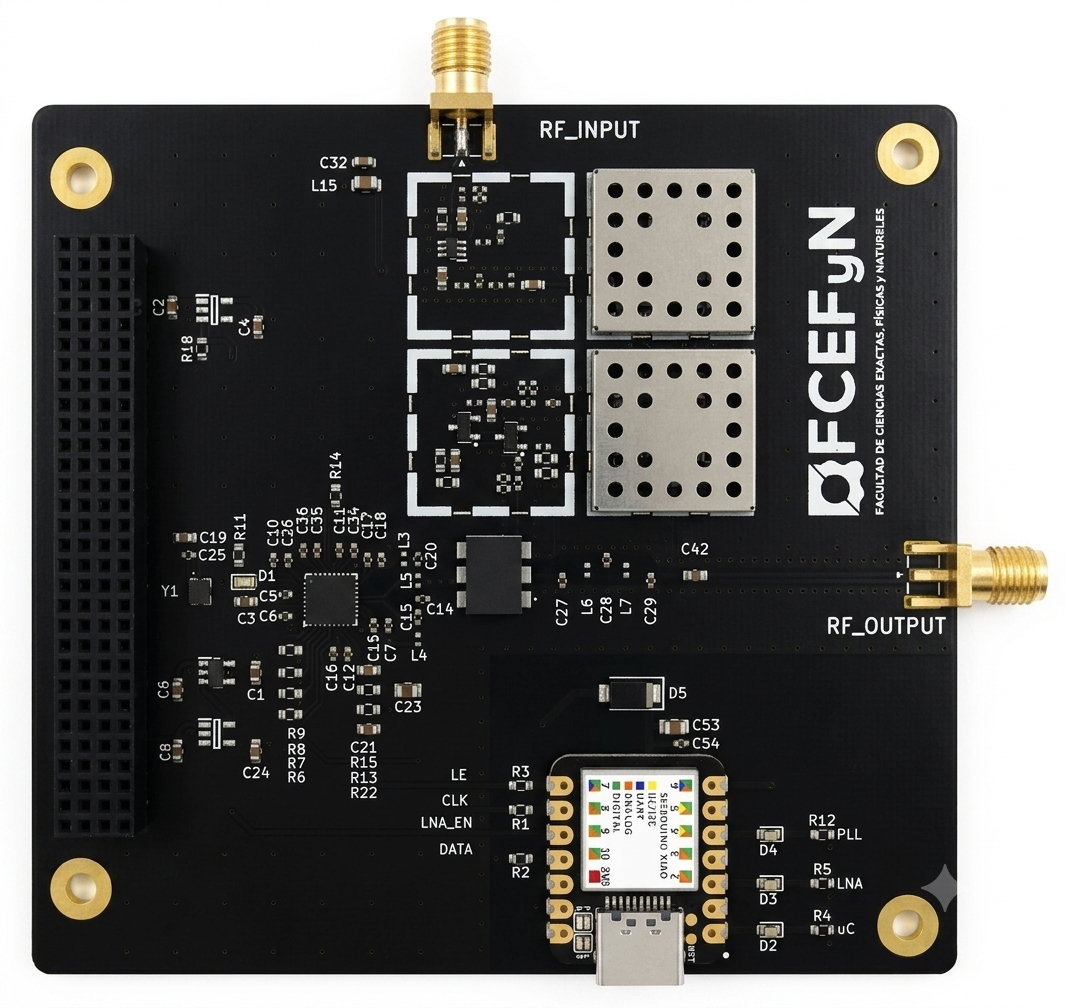
\includegraphics[width=0.8\linewidth]{imagenes/placa_kicad_3d}
		\caption[Diseño 3D en KICAD (Fuente: propia)]{Diseño 3D en KICAD (Fuente: propia)}
		\label{fig:placa3dkicad}
	\end{figure}
	
	\section{Antecedentes del problema}
	En los últimos años, el estándar CUBESAT ha democratizado el acceso al espacio, permitiendo a universidades e instituciones de investigación desarrollar misiones satelitales a costos reducidos. Sin embargo, a nivel local, no  existen antecedentes orientados al desarrollo integral y propio de un modulo transponder diseñado bajo requerimientos aeroespaciales. Tradicionalmente, la implementación de estos subsistemas ha dependido de módulos comerciales prefabricados, o desarrollos fuera de norma, lo que limita la apropiación de conocimientos en este campo.
	
	\section{Relevancia del trabajo}
	La relevancia de este trabajo radica en aportar al desarrollo tecnológico propio en el área de las comunicaciones aeroespaciales académicas. Al diseñar un hardware a nivel de componentes (etapa receptora y mezcladora), se genera un antecedente técnico y una base metodológica reutilizable para futuros desarrollos en la institución. Además, la compatibilidad con el factor de forma PC-104 garantiza la modularidad con otros subsistemas de la arquitectura satelital, mientras que la posibilidad de ser ensayado provee un medio de validación práctica.
	
	\section{Motivación para la elección del tema}
	La motivación principal surge de la necesidad de contar con plataformas locales, económicas y accesibles para la formación e investigación aplicada en el área de ingeniería de radiofrecuencia y sistemas espaciales. Este desarrollo permite acortar la brecha entre la teoría de los sistemas de telecomunicaciones y su implementación práctica en hardware con rigurosidad técnica.
	
	Asimismo, contar con un módulo transponder funcional abre un amplio abanico de aplicaciones prácticas en misiones de globos estratosféricos. Al operar como un repetidor lineal de banda ancha en frecuencias VHF-UHF, el sistema posibilita:
	
	\begin{itemize}
		\item \textbf{Retransmisión de comunicaciones entre estaciones terrenas:} Actuar como nodo de enlace para interconectar estaciones de radioaficionados o laboratorios universitarios distantes, aprovechando la amplia línea de vista que ofrece la estratosfera ($\sim$20--30 km) o una órbita LEO.
		
		\item \textbf{Comunicaciones de emergencia en zonas remotas:} Desplegar plataformas capaces de retransmitir señales de voz y datos en áreas afectadas por catástrofes naturales o sin cobertura de infraestructura terrestre.
		
		\item \textbf{Relevo de telemetría de sensores remotos (\textit{Data Relay}):} Recibir señales provenientes de estaciones de medición o sensores distribuidos en tierra y retransmitirlas hacia una estación terrestre para su procesamiento.
		
		\item \textbf{Validación de herencia de vuelo (\textit{Flight Heritage}):} Demostrar el correcto desempeño de la cadena de radiofrecuencia en condiciones operativas reales (baja presión, variaciones térmicas extremas y ambiente expuesto radiación ), elevando el nivel de madurez tecnológica (TRL, \textit{Technology Readiness Level}) del prototipo para futuras misiones espaciales institucionales.
	\end{itemize}
	
	\section{Formulación del problema}
	¿Cómo diseñar e implementar un módulo receptor y mezclador de RF en formato PC-104 que responda a los requerimientos de sensibilidad, frecuencia y ancho de banda para comunicaciones VHF-UHF en un CUBESAT, garantizando la integridad de señal y el cumplimiento de las restricciones electromecánicas a bajo costo?
	
	\section{Objetivo General y Objetivos Específicos}
	El objetivo general es diseñar, construir y validar experimentalmente un prototipo funcional de las etapas receptora y mezcladora de un transponder VHF-UHF bajo los estándares PC-104 y CUBESAT, asentando las bases para el desarrollo futuro de un transponder satelital completo. Para alcanzar el objetivo general, se plantean los siguientes objetivos específicos:
	\begin{itemize}
		\item Revisar y documentar las normas aplicables que puedan tener incidencias en el diseño (estándares CUBESAT y PC-104).
		
		\item Definir la arquitectura de RF del receptor, identificar y describir los bloques funcionales principales del transponder y su rol en la cadena de comunicación.
		
		\item Seleccionar componentes electrónicos adecuados considerando costo, disponibilidad, vida útil, tolerancias y desempeño en RF. Buscar distribuidores con disponibilidad de componentes y fabricantes de PCB (nacionales o internacionales) con la capacidad de fabricar en 4 capas a un bajo costo.
		
		\item Diseñar el esquema eléctrico y la placa de circuito impreso (PCB) aplicando buenas prácticas de integridad de señal y criterios de diseño en RF.
		
		\item Realizar simulaciones sobre el circuito eléctrico y su desempeño en RF, verificar ganancias, adaptación de impedancias, frecuencias de corte, reflexiones directas e inversas, polarización, estabilidad incondicional,etc.
		
		\item Montar el prototipo físico y realizar mediciones experimentales de los parámetros clave (sensibilidad, potencia, ancho de banda, figura de ruido e intermodulación).
		
		\item Documentar los resultados obtenidos y demostrar la viabilidad del transponder como carga útil para globos estratosféricos de aplicación académica y experimental.
	\end{itemize}
	
	\section{Metodología utilizada}
	Para el desarrollo de este trabajo se adopta la siguiente metodología:
	
	\begin{enumerate}
		\item \textbf{Fase de Análisis y Especificación:} Revisión bibliográfica de la normativa satelital (estándares CubeSat y PC-104), análisis de requerimientos y definición de las especificaciones teóricas de RF de la cadena receptora.
		
		\item \textbf{Fase de Diseño Teórico y Simulación:} Modelado circuital de los amplificadores y filtros utilizando herramientas SPICE, simulación de elementos de parámetros distribuidos y estimación teórica del desempeño de la cadena de recepción (ganancia, figura de ruido y selectividad).
		
		\item \textbf{Fase de Diseño de la PCB:} Layout de la placa de circuito impreso tomando como base una plantilla con factor de forma PC-104, aplicando reglas estrictas de integridad de señal y RF.
		
		\item \textbf{Fase de Implementación y Montaje:} Ensamble del prototipo físico mediante soldadura de componentes SMD.
		
		\item \textbf{Fase de Ensayos y Validación:} Caracterización y medición experimental utilizando instrumental especializado de RF (analizador de espectro, generador de señales de alta frecuencia), contrastando los resultados obtenidos frente a las simulaciones teóricas.
	\end{enumerate}\newpage
	
	% ==========================================
	% MARCO TEÓRICO
	% ==========================================
	\part{MARCO TEÓRICO}
	\chapter{Título del Marco Teórico}
	\section{Estándar CUBESAT}
	El CubeSat Design Specification (CDS) es el documento oficial de Cal Poly (versión vigente: Rev. 14.1, febrero 2022) que establece el conjunto de reglas que garantizan que cualquier CubeSat pueda ser lanzado de manera segura y compatible en un cohete comercial.
	Los lanzadores son los vehículos espaciales (cohetes) que transportan los CubeSats al espacio. La gran mayoría de CubeSats no viajan como carga primaria, sino como carga secundaria (piggyback) junto con satélites grandes.
	Para que esto sea posible, los CubeSats deben cumplir estrictamente con las dimensiones, masa y restricciones mecánicas/eléctricas definidas en el estándar, de modo que puedan ser integrados en un dispensador. El dispensador se instala en el lanzador y se encarga de guiar, contener y liberar a los CubeSats en la órbita asignada. Es importante discernir que, en el documento se utiliza tres \textbf{"Términos operativos"} diferentes a la hora de enumerar las distintas especificaciones:
	
	\begin{figure}[h!]
		\centering
		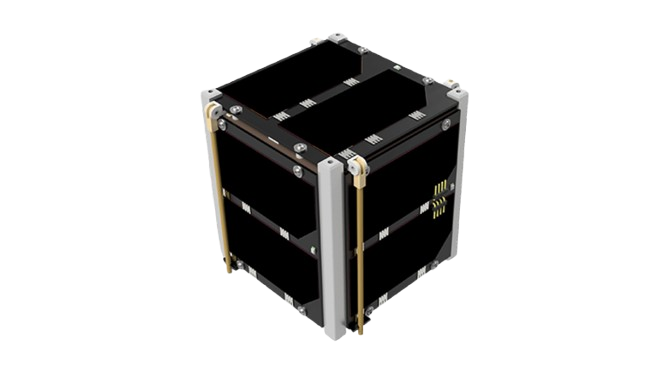
\includegraphics[width=1\linewidth]{imagenes/cubesat}
		\caption[Estándar CUBESAT (Fuente: medium.com)]{Estándar CUBESAT (Fuente: medium.com)}
		\label{fig:cubesat}
	\end{figure}
	
	\subsection{Especificaciones generales}
	\begin{enumerate}
		\item Todas las piezas deberán permanecer unidas a los CubeSats durante el lanzamiento, la eyección y el funcionamiento.
		
		\item Los artículos pirotécnicos deberán cumplir con AFSPCMAN 91-710(Volumen 3). 
		
		\item Todos los sistemas de propulsión deberán diseñarse, integrarse y probarse de acuerdo con AFSPCMAN 91-710(Volumen 3).
		
		\item Los sistemas de propulsión deberán tener al menos tres inhibidores de activación.
		
		\item Nota: Se recomienda tener en cuenta los requisitos de la Administración Federal de Aviación (FAA)  para las baterías transportadas por pasajeros de aerolíneas. La capacidad máxima permitida para baterías de iones de litio de tamaño estándar en el equipaje de mano es de 100 Wh por batería. 
		
		\item Los materiales peligrosos del CubeSat deberán cumplir con AFSPCMAN 91-710(Volumen 3).
		
		\item Los materiales de los CubeSats deberán cumplir con los criterios de baja desgasificación. Puede consultar una lista de materiales de baja desgasificación aprobados por la NASA 
		
		\subitem  Los materiales de los CubeSats deberán tener una pérdida de masa total (TML) inferior o igual al 1,0 \%.
		\subitem  Los materiales de los CubeSats deberán tener un material condensable volátil recolectado (CVCM) inferior o igual al 0,1 \%.
		
		\item El campo magnético de cualquier imán pasivo se limitará a $0,5$ Gauss por encima del campo magnético de la Tierra, fuera de la envoltura estática del CubeSat.
		
		\item El CubeSat deberá diseñarse para permitir ventilación durante el ascenso, de manera que la relación volumen ventilable/área de ventilación sea menor a 50,8 metros.
		
	\end{enumerate}
		
	\subsection{Especificaciones mecánicas}
	Los planos donde se especifican las dimensiones y características del CubeSat se pueden encontrar en la siguiente sección CDSDrawings2022
	
	\begin{enumerate}
		\item Nota: El Procedimiento de Inspección y Comprobación de Ajuste (CIFP) del CubeSat puede utilizarse para verificar que el CubeSat cumple con los requisitos dimensionales especificados.
		
		\item El origen del sistema de coordenadas del CubeSat se encuentra en el centro geométrico del CubeSat.
		
		\begin{figure}[h!]
			\centering
			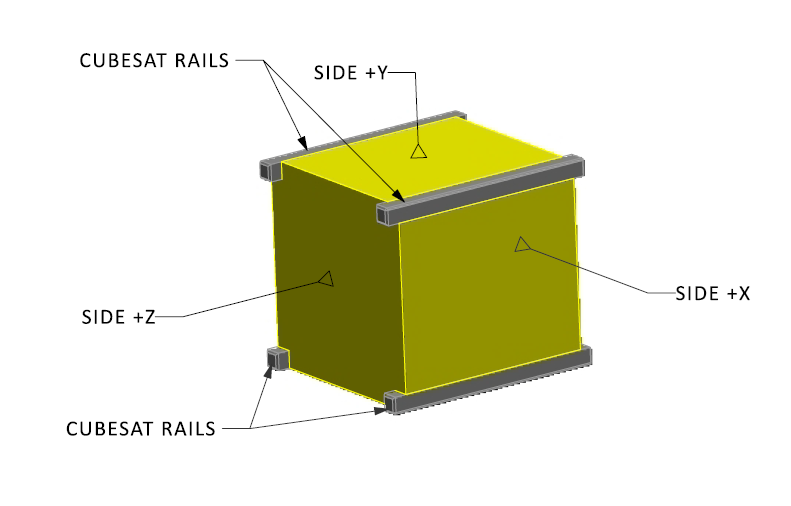
\includegraphics[width=0.7\linewidth]{imagenes/xyz_cubesat}
			\caption[Sistema de referencias CubeSat ejes coordenados (Fuente: CDSDrawings2022)]{Sistema de referencias CubeSat ejes coordenados (Fuente: CDSDrawings2022)}
			\label{fig:xyzcubesat}
		\end{figure}
		
		
		\item La configuración y las dimensiones físicas del CubeSat deberán cumplir con la sección correspondiente especificado en el plano.
		
		\item Nota: La dimensión de la longitud del separador de $5.0$ a $7.0$ mm con tolerancia de $0.1$ mm en la cara $\pm$ Z, especificada en los planos, existe para evitar interferencia con posibles CubeSats vecinos y con las interfaces del dispensador.Las caras $\pm$ Z son las que se orientan en el eje de eyección dentro del dispensador, por tanto, son las más críticas para asegurar que nada sobresalga más allá de lo permitido.
	
		\item Nota: Puede haber volumen adicional disponible para CubeSats de 3U, 6U y 12U. Este volumen adicional a veces se denomina volumen de la "lata de atún". La disponibilidad y las dimensiones del volumen dependen del dispensador.
		
		\item La cara –Z del CubeSat se insertará primero en el dispensador.
		
		\item Ningún componente de los lados sombreados en amarillo (ver dibujos del CDS) no debe sobresalir más de 6,5 mm normal a la superficie desde el plano del riel.
		
		\item Nota: Consulte el CIFP (CubeSat Inspection and Fit-check Procedure) para conocer la técnica de medición de protuberancia recomendada. Este consiste en un procedimiento oficial para verificar que un CubeSat cumple con las especificaciones mecánicas establecidas en el CubeSat Design Specification (CDS).
		
		\item Los elementos desplegables (antenas, paneles solares, booms, etc.) deberán estar asegurados por el propio CubeSat, no por el dispensador. Este requisito proviene de las exigencias de la mayoría de los proveedores de lanzamiento. La norma exige que sea el propio CubeSat quien asegure esos elementos.
		
		\item Los rieles deberán tener un ancho mínimo de 8,5 mm medido desde el borde del riel hasta la primera protuberancia en cada cara.
		
		\item Los rieles deben tener una rugosidad superficial menor a 1,6 um.
		
		\item Los bordes de los rieles deben redondearse con un radio de al menos 1 mm.
		
		\item Los extremos de los rieles en la cara  $\pm$ Z deberán tener una superficie mínima de 6,5 mm x 6,5 mm de área de contacto con los rieles del CubeSat vecinos.
		
		\item Al menos el 75$\%$ del riel debe estar en contacto con los rieles del dispensador. El 25$\%$ restante del riel puede estar empotrado (retraído).
		
		\item El cuadro  muestra la masa máxima típica para cada configuración en U. Las masas aceptables pueden variar según las capacidades del dispensador. Las masas superiores a la presentada en la cuadro pueden evaluarse misión por misión.
		
		\begin{table}[h!]
			\centering
			\renewcommand{\arraystretch}{1}
			\begin{tabular}{|c|c|}
				\hline
				Configuración U & Masa [Kg]   \\
				\hline
				1U   & 2.00  \\ \hline
				1.5U & 3.00  \\ \hline
				2U   & 4.00  \\ \hline
				3U   & 6.00  \\ \hline
				6U   & 12.00 \\ \hline
				12U  & 24.00 \\ \hline
			\end{tabular}
			\caption{Masa máxima permitida según configuración CubeSat (Fuente: CDS Rev. 14.1).}
			\label{tab:cubesat_mass}
		\end{table}
		
		\begin{figure}[h!]
			\centering
			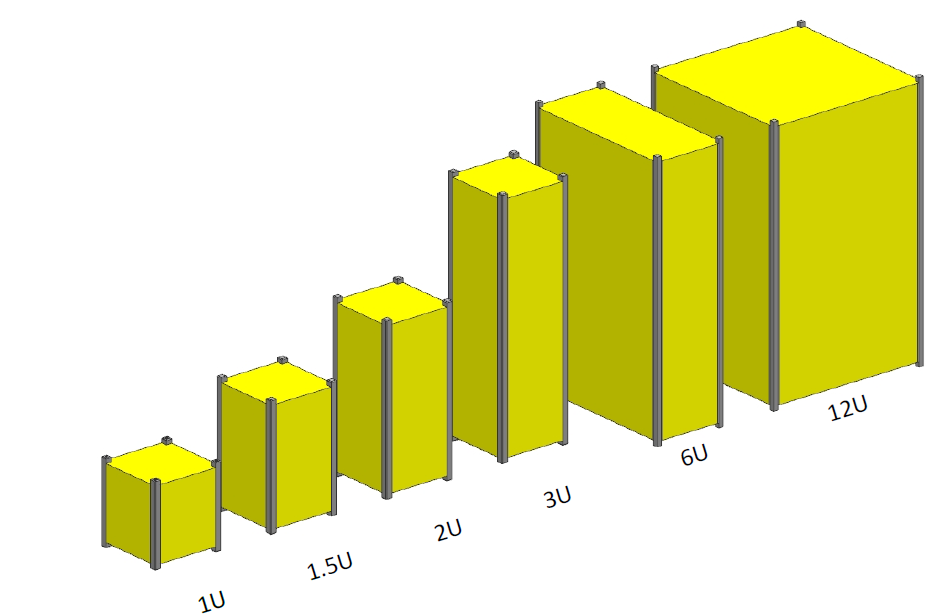
\includegraphics[width=0.7\linewidth]{imagenes/size_cubesat}
			\caption[Configuraciones en U(Fuente: CDSDrawings2022)]{Configuraciones en U(Fuente: CDSDrawings2022)}
			\label{fig:extravolcubesat}
		\end{figure}
		
		\item El centro de gravedad del CubeSat deberá estar dentro de los rangos especificados en el cuadro.
		
		\begin{table}[h!]
			\centering
			\renewcommand{\arraystretch}{1} % más espacio entre renglones
			\begin{tabular}{|c|c|c|c|}
				\hline
				Configuración U & Eje X & Eje Y & Eje Z \\
				\hline
				1U   & +2 cm / -2 cm & +2 cm / -2 cm & +2 cm / -2 cm \\ \hline
				1.5U & +2 cm / -2 cm & +2 cm / -2 cm & +3 cm / -3 cm \\ \hline
				2U   & +2 cm / -2 cm & +2 cm / -2 cm & +4.5 cm / -4.5 cm \\ \hline
				3U   & +2 cm / -2 cm & +2 cm / -2 cm & +7 cm / -7 cm \\ \hline
				6U   & +4.5 cm / -4.5 cm & +2 cm / -2 cm & +7 cm / -7 cm \\ \hline
				12U  & +4.5 cm / -4.5 cm & +4.5 cm / -4.5 cm & +7 cm / -7 cm \\
				\hline
			\end{tabular}
			\caption{Rangos aceptables de ubicación del centro de gravedad medidos desde el centro geométrico en cada eje principal (Fuente: CDS Rev. 14.1).}
			\label{tab:centro_gravedad}
		\end{table}
		
		\item La estructura del CubeSat debe estar hecha de aleación de aluminio. Normalmente, se utiliza aluminio 7075, 6061, 6082, 5005 o 5052 tanto para la estructura principal del CubeSat como para los rieles.
		
		\item Cualquier superficie externa de aluminio del CubeSat, como los rieles y separadores que estén en contacto con los rieles del dispensador, deberá estar anodizada.\newpage
		
		\item Si un CubeSat comparte un dispensador con otro(s) CubeSat(s), cada CubeSat deberá emplear un mecanismo que favorezca la separación respecto de los CubeSats vecinos dentro del dispensador. Cualquier mecanismo que proporcione separación es aceptable, resortes, imanes, etc.
		
		\item El mecanismo de separación no deberá extenderse más allá del nivel del separador (standoff) en configuración almacenada (stowed configuration).
		
		\item Nota: La ubicación más común del mecanismo de separación del CubeSat es centrada en el extremo de los dos standoffs de la cara –Z del CubeSat.
		
		\item Nota: No se requiere un mecanismo de separación para CubeSats que no compartan un dispensador con otro(s) CubeSat(s).
	\end{enumerate}
	
	
	
	\subsection{Especificaciones eléctricas}
	Los sistemas electrónicos se diseñarán con las siguientes características de seguridad.
	\begin{enumerate}
		\item Para evitar que el CubeSat active cualquier función que requiera energía, el sistema de potencia del CubeSat deberá permanecer en estado apagado desde el momento de la entrega al vehículo de lanzamiento hasta el despliegue en órbita.
		
		\item Nota: Las funciones alimentadas del CubeSat incluyen la variedad de subsistemas como C\&DH, comunicación por RF,ADC, activación de mecanismos desplegables, etc. Los sistemas de potencia del CubeSat incluyen todos los conjuntos de baterías y celdas solares.
		
		\item Los CubeSats deberán incorporar protección de circuito de batería para la carga/descarga con el fin de evitar condiciones de celdas desbalanceadas. Se requerirá documentación adicional del fabricante y/o ensayos para celdas modificadas, personalizadas o que no estén certificadas bajo UL (Underwriters Laboratories), norma de seguridad internacional.
		
		\item El CubeSat deberá tener, como mínimo, un interruptor de despliegue (deployment switch), el cual se acciona mientras está integrado en el dispensador. Este mantiene el satélite apagado mientras esté dentro del dispensador. Solo al ser liberado en órbita este interruptor se desactiva, permitiendo encender el sistema de manera segura.
		
		\item En el estado activado, el interruptor de despliegue del CubeSat desconectará eléctricamente el sistema de energía de las funciones alimentadas.
		
		\item El interruptor de despliegue deberá estar en estado activado en todo momento mientras esté integrado en el dispensador.
		
		\item En estado activado, el interruptor de despliegue del CubeSat debe estar al nivel o por debajo de cualquier superficie externa que interactúe con el dispensador o el CubeSat adyacente. Esto garantiza que el interruptor no dañe ni interfiera con la superficie de contacto.
		
		\item Si el interruptor de despliegue del CubeSat cambia del estado activado al estado anterior al lanzamiento, el satélite se restablecerá a un estado previo al lanzamiento, lo que incluye el reinicio de la transmisión y los temporizadores.
		
		\item Se podrán permitir los relojes de tiempo real (RTC) si cumplen los requisitos:
		
		\subitem  Los circuitos RTC deberán estar aislados del sistema de alimentación principal.
		\subitem  Las frecuencias RTC deberán ser inferiores a 320 kHz
		\subitem  Los circuitos RTC deberán tener una corriente limitada a menos de 10 mA.
		
		\item El pin RBF (Remove Before Flight) y todos los conectores umbilicales del CubeSat deberán estar dentro de las ubicaciones de puertos de acceso designados, si estos están disponibles en el dispensador del CubeSat.
		
		\item Nota: Algunos dispensadores no tienen puertos de acceso, por lo que es necesario retirar el RBF antes de insertarlo en el dispensador. Se recomienda que el desarrollador del CubeSat tenga en cuenta esta posibilidad al diseñar la secuencia de encendido y arranque.
		
		\item El CubeSat incluirá un pin RBF, que corta toda la energía al satélite una vez que se inserta en él.
		
		\item El pin RBF deberá retirarse del CubeSat antes de la integración en el dispensador, si este no dispone de puertos de acceso.
		
		\item El CubeSat deberá tener al menos tres inhibidores de RF independientes para impedir la transmisión de RF involuntaria.
		
		\item Nota: Un inhibidor es un dispositivo físico entre una fuente de energía y un peligro.
		
		\item Nota: Un temporizador no se considera un inhibidor independiente.
		
		\item Nota: Algunos proveedores de vehículos de lanzamiento solo requerirán uno o dos inhibidores independientes, dependiendo de la potencia de RF del CubeSat. Sin embargo, se recomienda encarecidamente el uso de tres inhibidores independientes, lo que puede reducir la documentación y los análisis necesarios.
		
		\item El CubeSat tendrá al menos tres inhibidores independientes para impedir la liberación accidental de cualquier estructura desplegable, como antenas o paneles solares.
	\end{enumerate}
	
	
	
	\subsection{Especificaciones operacionales}
	Los CubeSats cumplirán ciertos requisitos de integración y funcionamiento para cumplir con las obligaciones legales y garantizar la seguridad de otros CubeSats.
	\begin{enumerate}
		\item Los operadores deberán obtener y proporcionar la documentación correspondiente de las licencias correspondientes para el uso de radiofrecuencias.
		
		\item Nota: Para el uso de frecuencias de radio-aficionado, se requiere un comprobante de coordinación de frecuencias emitido por la IARU.
		
		\item Los CubeSats deberán cumplir con los acuerdos y restricciones de licencia de radio de su país. (ver normas del ENACOM)
		
		\item Nota: El operador de CubeSat debe consultar a la Unión Internacional de Telecomunicaciones (UIT) para determinar qué licencias y aprobaciones necesita en su país.
		
		\item El diseño y el hardware de la misión CubeSat deberán cumplir con la norma NPR 8715.6  para limitar los desechos orbitales.
		
		\item Cualquier componente del CubeSat deberá reingresar con una energía inferior a 15 julios.
		
		\item Los desarrolladores deben estar preparados para proporcionar datos de mitigación de desechos orbitales si así lo solicita la agencia de licencias o el proveedor de lanzamiento.
		
		\item Nota: La Agencia Espacial Europea (ESA) ofrece un software de evaluación de residuos en ESA\_SDUP2025.
		
		\item Todos los elementos desplegables, como brazos, antenas y paneles solares, deberán esperar un mínimo de 30 minutos para desplegarse después de que se activen los interruptores de despliegue del CubeSat durante la eyección del dispensador.
		
		\item Los CubeSats no generarán ni transmitirán una señal antes de 45 minutos después de su despliegue en órbita.
		
		\item Nota: El CubeSat se puede encender inmediatamente después del despliegue desde el dispensador.
		
		\item Nota: Las entidades privadas (no pertenecientes al gobierno estadounidense) bajo la jurisdicción o control de Estados Unidos que se propongan operar un sistema espacial de teledetección (satélite), como un generador de imágenes visuales, podrían necesitar una licencia de teledetección, según lo exige la legislación estadounidense.
		
		\item El desarrollador del dispensador llevará a cabo al menos una prueba de ajuste (fit check), en la cual la unidad de vuelo del CubeSat será inspeccionada e integrada en el dispensador o en un dispensador de ingeniería (réplica) para verificar el encaje. Una prueba de ajuste final se realizará justo antes de la integración de la unidad de vuelo del CubeSat en el dispensador.
	\end{enumerate}
	
	\subsection{Requerimientos de prueba}
	Todos los niveles y requisitos de ensayo son específicos de cada misión y varían en cada lanzamiento. Los ejemplos proporcionados en este documento son, típicamente, los más estrictos, con el fin de abarcar los requisitos de la mayoría de las oportunidades de lanzamiento hasta la fecha. Los ensayos se realizarán para cumplir con los requisitos del proveedor de lanzamiento, así como con cualquier requisito adicional considerado necesario para garantizar la seguridad de los CubeSats, el dispensador y la carga útil primaria del vehículo de lanzamiento. Si el entorno del vehículo de lanzamiento es desconocido, se puede utilizar el General Environmental Verification Standard (GEVS, GSFC-STD-7000A) y el SMC-S-016 para definir los entornos y requisitos de ensayo. Cabe señalar que los niveles de ensayo definidos en GSFC-STD-7000A y SMC-S-016 no garantizan abarcar o satisfacer todos los entornos de ensayo de vehículos de lanzamiento. Normalmente, todos los CubeSats deberán someterse a los siguientes ensayos:
	\begin{enumerate}
		\item \textbf{Vibración aleatoria}: El ensayo de vibración aleatoria se realizará a los niveles y durante el tiempo definido por el proveedor de lanzamiento.
		
		\item \textbf{Horneado en vacío térmico (Thermal Vacuum Bakeout)}. Se realizará un horneado en vacío térmico para garantizar la desgasificación adecuada de los componentes. La especificación de este ensayo será definida por el proveedor de lanzamiento.
		
		\item \textbf{Ensayo de choque (Shock Testing)}: El ensayo de choque se realizará según lo definido por el proveedor de lanzamiento.Normalmente, los CubeSats no requieren ensayo de choque.
		
		\item \textbf{Inspección visual}: Se realizará una inspección visual del CubeSat y la medición de áreas críticas de acuerdo con el CIFP (cubesat.org) o según lo definido por el proveedor de lanzamiento.
	\end{enumerate}
	
	\section{Estándar PC-104}
	En el documento (PC-104 Specification Version 2.6 October 13, 2008) proporciona las especificaciones mecánicas y eléctricas. En el ámbito de desarrollo de CubeSats es una práctica estándar adoptar únicamente la geometría mecánica del estándar PC-104 (dimensiones de placa, agujeros de montaje y formato de conector) mientras se define una asignación de pines (pinout) totalmente personalizada adaptada a microcontroladores ARM y a las necesidades del satélite. La especificación eléctrica original del bus ISA de 16 bits (así como PCI/PCIe en PC/104-Plus) no se aplica en arquitecturas de subsistemas espaciales modernos.
	
	\begin{figure}[h!]
		\centering
		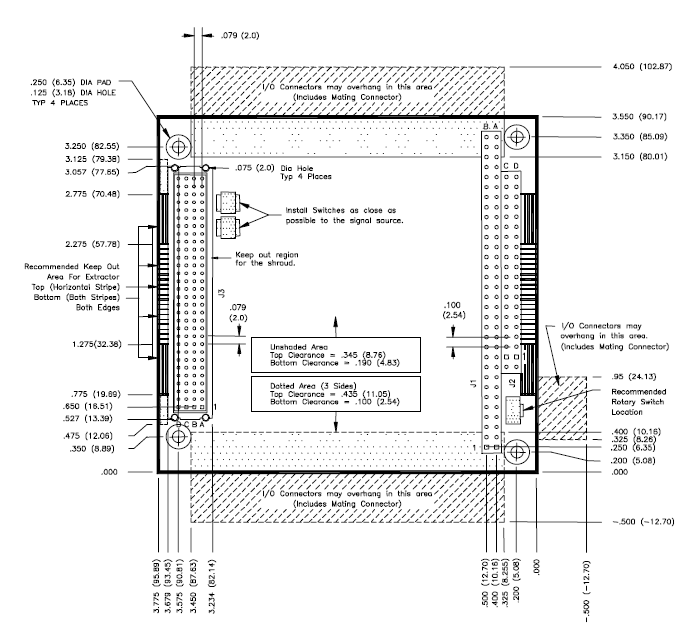
\includegraphics[width=0.8\linewidth]{imagenes/mec_pc104p}
		\caption[Dimensiones del modulo para bus de 8 bits (Fuente: PC-104 Specification)]{Dimensiones del modulo para bus de 8 bits (Fuente: PC-104 Specification)}
		\label{fig:dimpc104}
	\end{figure}\newpage
	
	\begin{figure}[h!]
		\centering
		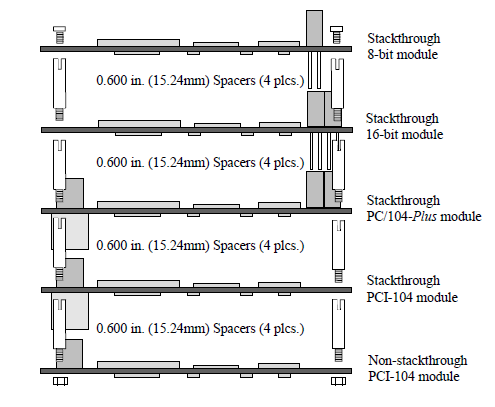
\includegraphics[width=0.75\linewidth]{imagenes/stack_pc104_p}
		\caption[Apilamientos de modulos de 8 y 16 bits (Fuente: PC-104 Specification)]{Apilamientos de modulos de 8 y 16 bits (Fuente: PC-104 Specification)}
		\label{fig:stackpc104}
	\end{figure}
	
	
	\section{Transpondedor Satelital}
	\subsection{Definición y principio de funcionamiento}
	Un transpondedor (transponder, acrónimo de TRANSmitter + resPONDER) es el componente central de la carga útil (payload) de comunicaciones de un satélite. Su función principal es recibir la señal enviada desde una estación terrestre (enlace de subida o uplink), procesarla para acondicionarla y retransmitirla hacia la Tierra (enlace de bajada o downlink).Un transpondedor actúa como un puente de radiofrecuencia. Debido a que las señales sufren pérdidas extremas en su viaje por el espacio (pérdidas por trayectoria en espacio libre o Free Space Path Loss), la señal que llega al satélite es sumamente débil (del orden de los picowatts o nanowatts).\newline
	
	La conversión de frecuencia entre el enlace de subida (uplink) y de bajada (downlink) es indispensable para desacoplar la entrada y la salida del repetidor, evitando que la señal de alta potencia retransmitida se filtre o realimente en el receptor. Sin embargo, realizar esta conversión directamente al inicio mediante un mezclador (front-end mixer) degradaría inaceptablemente la temperatura de ruido global del sistema debido a la elevada figura de ruido que poseen los mezcladores. El LNA establece la temperatura efectiva de ruido del sistema a la frecuencia de subida y aporta una ganancia elevada (típicamente entre $20dB$ y $40dB$), la cual enmascara y minimiza la contribución de ruido del mezclador que se ubica justo después. Posterior al LNA, el mezclador junto al oscilador local realiza el cambio de frecuencia, posicionándose en un punto estratégico de la cadena donde el nivel de la señal sea lo suficientemente alto respecto al ruido, pero controlado para no activar efectos no lineales en el componente.\newline
	
	Tras la conversión de frecuencia, y teniendo en cuenta la ganancia del amplificador de bajo ruido y las pérdidas de conversión del mezclador, aún queda por proporcionar cierta cantidad de ganancia para obtener la ganancia total de potencia requerida. Dependiendo de las bandas de frecuencia involucradas, las consideraciones tecnológicas pueden dificultar la obtención de una alta ganancia de potencia a la frecuencia del enlace de bajada (downlink). En estos casos, se utiliza una doble conversión de frecuencia mediante una frecuencia intermedia (IF) de menor valor que la frecuencia de bajada. Las señales del enlace de subida (uplink) se convierten primero de forma descendente a la IF, donde se realiza la amplificación. Luego, un conversor ascendente traslada la frecuencia a la del enlace de bajada.
	
	\begin{figure}[h!]
		\centering
		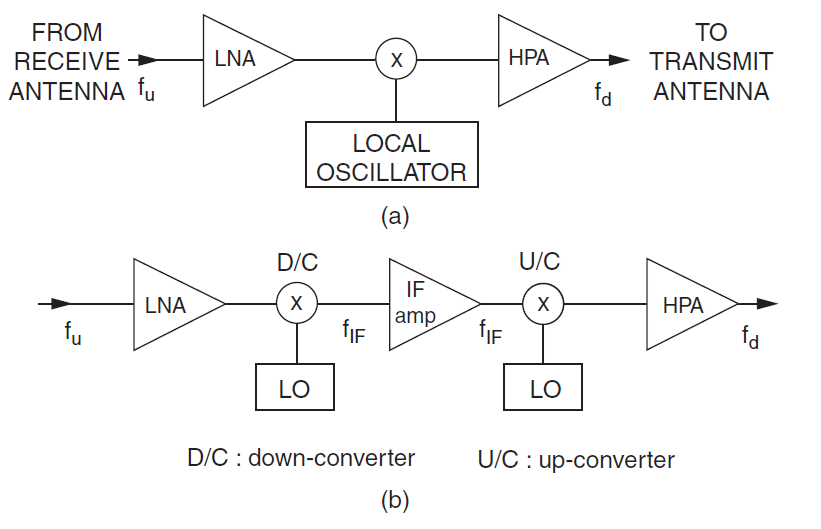
\includegraphics[width=0.65\linewidth]{imagenes/tranponder_1}
		\caption[Conversion simple vs conversion doble (Fuente: Maral, G., Bousquet, M, Z.)]{Conversion simple vs conversion doble (Fuente: Maral, G., Bousquet, M., Z. Satellite Communications Systems)}
		\label{fig:tranponder1}
	\end{figure}
	
	Algunos sistemas incluyen demultiplexado e IMUX (Input Multiplexer), el ancho de banda total del satélite se divide mediante un banco de filtros en múltiples canales individuales, ademas de multiplexado de Salida (OMUX): Los canales ya amplificados se vuelven a combinar en un solo canal utilizando filtros de alta potencia.
	
	\begin{figure}[h!]
		\centering
		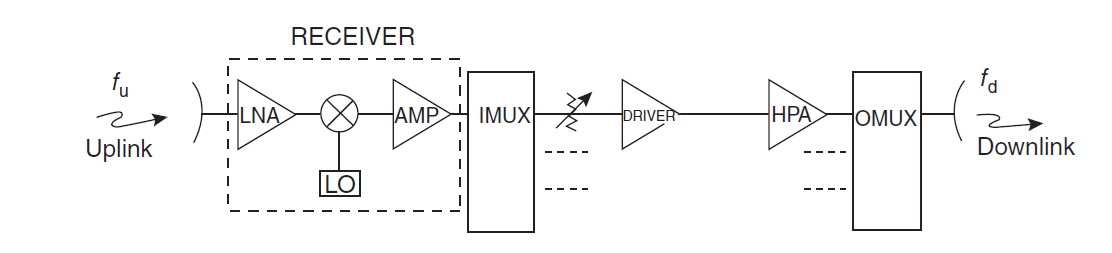
\includegraphics[width=1\linewidth]{imagenes/transponder_2}
		\caption[Organizacion general de un transponder (Fuente: Maral, G., Bousquet, M., Z.)]{Organizacion general de un transponder (Fuente: Maral, G., Bousquet, M., Z. Satellite Communications Systems)}
		\label{fig:transponder2}
	\end{figure}
	
	\subsection{Tipos de transpondedores: Regenerativos vs. Transparentes (Lineales)}
	El repetidor transparente, conocido como de tipo bent-pipe o tubo curvado, opera mediante un procesamiento $100\%$ analógico en el que la señal de subida (uplink) es recibida, filtrada, convertida en frecuencia mediante un oscilador local para evitar la auto-interferencia y amplificada en potencia antes de ser retransmitida hacia la Tierra.
	
	\begin{figure}[h!]
		\centering
		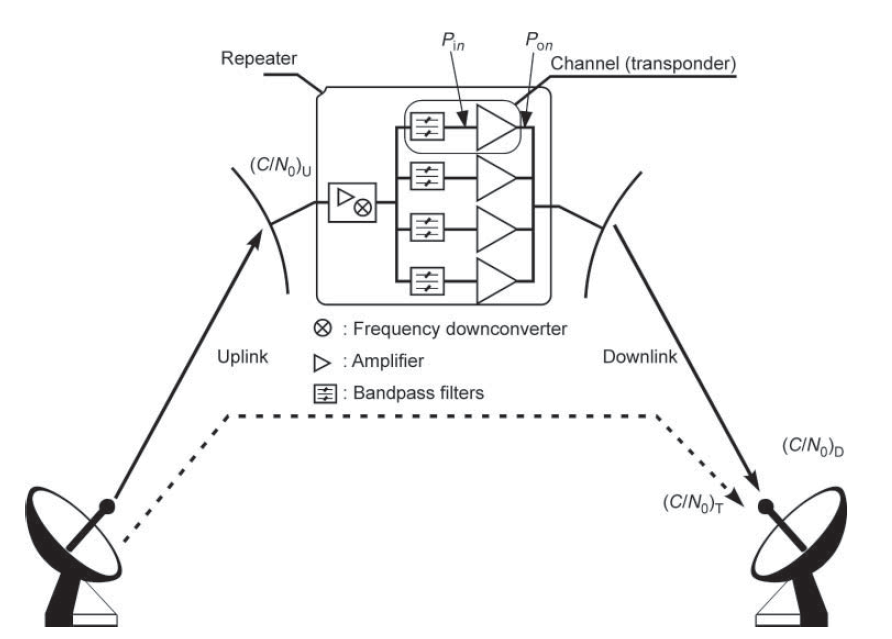
\includegraphics[width=0.65\linewidth]{imagenes/transponder_3}
		\caption[Enlaces up-link VHF y down-link UHF (Fuente: Maral, G., Bousquet, M., Z.)]{Enlaces up-link VHF y down-link UHF (Fuente: Maral, G., Bousquet, M., Z. Satellite Communications Systems)}
		\label{fig:transponder3}
	\end{figure}
	Su ventaja principal reside en su absoluta independencia o transparencia respecto al protocolo de comunicación, el tipo de modulación o la tasa de datos empleada, lo que permite actualizar libremente la tecnología de las estaciones terrestre durante la vida útil del satélite sin modificar el hardware, ofreciendo además una latencia casi nula, menor consumo energético y alta confiabilidad. Sin embargo, su mayor desventaja es la acumulación inevitable de ruido e interferencias: el transpondedor no distingue entre la señal útil y las degradaciones captadas en el trayecto, amplificando el ruido del enlace de subida de forma conjunta con la información. Asimismo, al manejar múltiples portadoras simultáneas, sufre distorsiones por intermodulación en sus amplificadores de potencia, obligando a operar el sistema con un margen de reducción de potencia (back-off) que disminuye la eficiencia energética global del satélite.\newline
	
	Por su parte, el repetidor regenerativo integra procesamiento digital a bordo (On-Board Processing - OBP) para demodular la señal analógica entrante hasta recuperar la secuencia de bits original en banda base, aplicando algoritmos de corrección de errores hacia adelante (FEC) para regenerar y limpiar completamente los datos antes de volver a modularlos y amplificarlos para el enlace de bajada.
	 
	Su ventaja determinante es la interrupción de la cadena de acumulación de ruido, ya que desacopla totalmente el desempeño del uplink respecto al downlink, entregando una señal retransmitida limpia y permitiendo cambiar los esquemas de modulación entre tramos, así como realizar enrutamiento o conmutación inteligente de paquetes entre distintos haces (beam switching). No obstante, sus desventajas radican en un incremento sustancial en la masa, el costo, la complejidad del hardware y el consumo energético del satélite, sumado a una mayor latencia provocada por el tiempo de procesamiento digital y una rigidez tecnológica severa, puesto que la plataforma queda irrevocablemente limitada a los protocolos y estándares digitales para los cuales fue programada antes de su lanzamiento.
	
	\begin{figure}[h!]
		\centering
		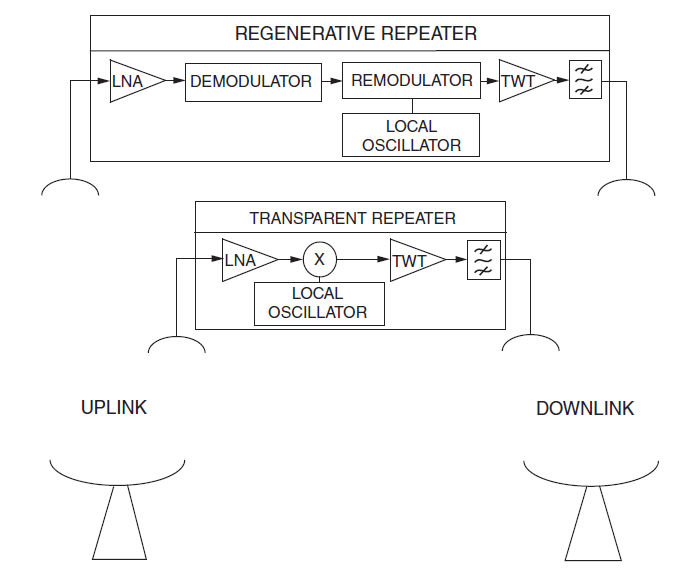
\includegraphics[width=0.7\linewidth]{imagenes/transponder_4}
		\caption[Transponder transparente vs regenerativo (Fuente: Maral, G., Bousquet, M., Z.)]{Transponder transparente vs regenerativo (Fuente: Maral, G., Bousquet, M., Z. Satellite Communications Systems)}
		\label{fig:transponder4}
	\end{figure}\newpage
	
	
	\section{Bloques Funcionales de Radiofrecuencia}
	\subsection{Amplificador de Bajo Ruido (LNA)}
	Para entender la imperiosa necesidad de colocar un Amplificador de Bajo Ruido (LNA) como primer bloque activo —antes de cualquier mezclador o etapa de conversión— es necesario recurrir al análisis de la acumulación de ruido térmico en sistemas multietapa mediante la formulación de Friis.
	Todo componente electrónico a una temperatura física $T$ genera ruido térmico. En telecomunicaciones satelitales, el ruido aportado por un bloque funcional se modela mediante su Temperatura Equivalente de Ruido ($T_e$) o su Factor de Ruido ($F$). La relación fundamental entre ambos parámetros está dada por:
	
	\begin{equation}
		T_e = T_0 (F - 1)
	\end{equation}
	
	donde $T_0 = 290K$ es la temperatura de referencia estándar.
	
	Cuando varios dispositivos (LNA, mezclador, amplificadores intermedios) se conectan en cascada, la temperatura equivalente de ruido total del receptor ($T_e$) vista desde la entrada de la antena no es la simple suma de los ruidos individuales, sino que se rige por la Ecuación de Friis para temperaturas de ruido:
	
	\begin{equation}
		T_e = T_1 + \frac{T_2}{G_1} + \frac{T_3}{G_1 G_2} + \frac{T_4}{G_1 G_2 G_3} + \dots
	\end{equation}
	
	En esta expresión, $T_i$ representa la temperatura equivalente de ruido del bloque $i$, y $G_i$ es la ganancia en potencia lineal (no en dB) del bloque $i$.\newpage
	
	Analizando la cadena de recepción típica de un repetidor satelital, la etapa de entrada está compuesta por: LNA con ganancia elevada $G_{LNA}$ y baja temperatura de ruido $T_{LNA}$, Mezclador (Mixer) con ganancia $G_{mix}$ (que en la práctica suele ser una pérdida, $G_{mix} < 1$) y una alta temperatura de ruido $T_{mix}$. Etapa de frecuencia intermedia o amplificación posterior con temperatura $T_{IF}$ y ganancia $G_{IF}$. Sustituyendo estos bloques en la fórmula de Friis para los dos primeros componentes críticos:
	
	\begin{equation}
		T_e = T_{LNA} + \frac{T_{mix}}{G_{LNA}} + \frac{T_{IF}}{G_{LNA} \cdot G_{mix}}
	\end{equation}
	
	Si se intentara realizar la conversión de frecuencia directamente a la entrada mediante un mezclador pasivo (front-end mixer) sin un LNA previo, la ganancia inicial sería menor a la unidad ($G_1 = G_{mix} < 1$). Esto provocaría que el ruido de todas las etapas posteriores se multiplicara en lugar de dividirse, disparando la temperatura total de ruido del receptor a niveles inaceptables.
	
	Al intercalar un LNA con una ganancia muy alta (típicamente $G_{LNA} = 20dB$ a $40dB$, equivalente a un factor lineal de $100$ a $10.000$), el término divisor $G_{LNA}$ reduce drásticamente el impacto de $T_{mix}$ y de las etapas subsecuentes. Matemáticamente:
	
	\begin{equation}
		G_{LNA} \gg 1  \longrightarrow \frac{T_{mix}}{G_{LNA}} \approx 0
	\end{equation}
	
	Por lo tanto, la temperatura equivalente de ruido de todo el receptor satelital queda enmascarada y reducida casi exclusivamente al ruido intrínseco del LNA:
	
	\begin{equation}
		T_e \approx T_{LNA}
	\end{equation}
	
	La calidad de la recepción de la carga útil no depende únicamente de la temperatura de la PCB o del receptor, sino de la Temperatura del Sistema ($T_{sys}$), la cual combina el ruido captado por la antena receptora del satélite ($T_{ant}$) y el ruido propio del receptor ($T_e$):
	
	\begin{equation}
		T_{sys} = T_{ant} + T_e \approx T_{ant} + T_{LNA}
	\end{equation}
	
	La potencia de ruido térmico total ($N$) presente en la entrada del repetidor en un ancho de banda de medida $B$ se calcula mediante la constante de Boltzmann ($k = 1.38 \times 10^{-23}J/K$):
	
	\begin{equation}
		N = k \cdot T_{sys} \cdot B
	\end{equation}
	
	De esta forma, minimizar $T_{LNA}$ minimiza directamente la potencia de ruido $N$ en el satélite.
	
	La capacidad del satélite para captar señales débiles se mide a través de su Figura de Mérito del Receptor ($G/T$), definida como la razón entre la ganancia de la antena receptora ($G_{rx}$) y la temperatura de ruido del sistema ($T_{sys}$):
	
	\begin{equation}
		\left(\frac{G}{T}\right) = \frac{G_{rx}}{T_{sys}} \quad [dB/K]
	\end{equation}
	
	Esta figura de mérito determina directamente la Relación Portadora-a-Ruido del enlace de subida $(C/N)_{up}$:
	
	\begin{equation}
		\left(\frac{C}{N}\right)_{up} = \frac{EIRP_{earth} \cdot \left(\frac{G}{T}\right)}{k \cdot B \cdot FSPL_{up}}
	\end{equation}
	
	Donde $EIRP_{earth}$ es la potencia transmitida desde la Estación Terrena y $FSPL_{up}$ representa las pérdidas por trayectoria en espacio libre. Como se observa en la formulación, si el LNA no tuviera una figura de ruido ultra baja, $T_{sys}$ aumentaría, lo que degradaría el cociente $(C/N)_{up}$. Para compensar dicha degradación sin un LNA adecuado, las estaciones terrenas se verían obligadas a aumentar drásticamente su potencia de emisión ($EIRP_{earth}$) mediante transmisores más grandes y costosos.
	
	Intentar suministrar semejante ganancia en una sola etapa o a una sola frecuencia causaría realimentaciones electromagnéticas parasitarias, provocando que el amplificador auto-oscile y quede inoperativo. La arquitectura propuesta resuelve esto dividiendo la ganancia: el LNA entrega los primeros $20dB$ a la frecuencia de subida ($f_{up}$) garantizando un piso de ruido bajo, el mezclador desplaza la frecuencia a una frecuencia intermedia o de bajada ($f_{down}$), y las etapas posteriores suministran los $60dB$ de ganancia restantes en esa nueva frecuencia. De esta manera se logra estabilidad global en la cadena de RF sin comprometer la figura de ruido.
	

	\subsection{Mezclador (\textit{Mixer}) y productos de conversión}
	Un mezclador de radiofrecuencia (RF) es un dispositivo no lineal o de parámetros variables en el tiempo que realiza la traslación espectral de una señal de entrada mediante la multiplicación con una señal de referencia suministrada por un Oscilador Local (LO).
	
	El principio del mezclador se fundamenta en la multiplicación en el dominio del tiempo de dos señales sinusoidales: la señal de entrada $v_{RF}(t) = A_{RF} \cos(\omega_{RF} t + \phi)$ y la señal del oscilador local $v_{LO}(t) = A_{LO} \cos(\omega_{LO} t)$.
	
	Por identidades trigonométricas, el producto de ambas señales genera dos componentes espectrales a la salida:
	\begin{equation}
		v_{out}(t) = k \cdot v_{RF}(t) \cdot v_{LO}(t) = \frac{k A_{RF} A_{LO}}{2} \left[ \cos((\omega_{RF} - \omega_{LO})t + \phi) + \cos((\omega_{RF} + \omega_{LO})t + \phi) \right]
	\end{equation}
	
	Parámetros importantes para el desempeño del mixer:
	\begin{itemize}
		\item \textbf{Ganancia / Pérdida de Conversión ($G_c$ / $L_c$)}: Relación entre la potencia de la señal de salida a la Frecuencia Intermedia (IF) y la potencia de la señal de entrada (RF):
		\begin{equation}
			L_c[dB] = P_{IF}[dBm] - P_{RF}[dBm]
		\end{equation}
		La supresión de las bandas laterales. En una conversión se producen dos bandas
		laterales. Los fabricantes especifican las pérdidas con una sola banda lateral. 
		\begin{equation}
			L_{cSSB}[dB] = L_{cDSB}[dB] +3[dB]
		\end{equation}
		
		\item \textbf{Figura de Ruido ($NF$)}: Incremento en la relación señal a ruido ($SNR$) debido al ruido térmico y de parpadeo intrínseco del mezclador. En mezcladores pasivos, la figura de ruido de banda lateral única (SSB) se aproxima linealmente a sus pérdidas de conversión ($NF_{SSB} \approx L_c$).\newpage
		
		\item \textbf{Punto de Compresión a 1 dB ($P_{1dB}$)}: Indica el límite superior del régimen de linealidad, donde la potencia de salida cae 1 dB respecto a la respuesta ideal.Normalmente en los mezcladores se especifica el punto en donde la compresión del nivel de entrada es de 1 dB o 3 dB (denotado como P1dB o P3dB, respectivamente)
		
		\item \textbf{Punto de Intersección de Tercer Orden ($IP3$)}: Parámetro de linealidad que cuantifica la generación de productos de intermodulación de tercer orden ($IMD_3$) producidos por dos tonos adyacentes ($2f_1 - f_2$ y $2f_2 - f_1$).
		
		\item \textbf{Rango Dinámico Libre de Espurias ($SFDR$)}: Margen de potencia entre la señal mínima detectable (piso de ruido) y el nivel donde los productos $IMD_3$ se igualan a dicho piso:
		\begin{equation}
			SFDR = \frac{2}{3} (IIP3 - SMD)
		\end{equation}
		
		Donde:
		\begin{equation}
			SMD [dBm] = -174 + log (BHz) + NF
		\end{equation}
		
		\item \textbf{Aislamiento entre Puertos (Port Isolation)}: Pérdida de inserción directa entre puertos ($I_{LO-RF}$, $I_{LO-IF}$, $I_{RF-IF}$). Valores típicos oscilan entre 30 dB y 60 dB. 
	\end{itemize}
	
	La Distorsión por Intermodulación (IMD) ocurre al aplicar dos o más señales en el puerto de entrada de un mezclador (usualmente analizada con dos tonos cercanos $f_{RF1}$ y $f_{RF2}$), las cuales reaccionan con la característica no lineal del dispositivo y con el oscilador local ($f_{LO}$). Esto genera componentes espurias de frecuencia expresadas como:
	
	\begin{equation}
		f_{espuria} = (\pm m f_{RF1} \pm n f_{RF2}) \pm f_{LO}
	\end{equation}
	
	La potencia de salida total $P_o$ afectada por la no linealidad se modela mediante una serie de potencias, donde $P_{in}$ es la potencia de entrada, $G_c$ es la ganancia o pérdida de conversión y $n$ representa el orden de la intermodulación:
	
	\begin{equation}
		P_o[W] = G_c (a_1 P_{in} + a_2 P_{in}^2 + a_3 P_{in}^3 + \dots + a_n P_{in}^n)
	\end{equation}
	
	En escala logarítmica, la respuesta para un producto de orden $n$ se describe mediante la recta:
	\begin{equation}
		P_o[dBm] = K_n[dB] + n P_{in}[dBm]
	\end{equation}
	
	Siendo $K_n = G[dB] + a_n$)
	
	Esta relación permite calcular la relación entre la potencia de entrada, el rango medio de intermodulación ($IMR$) y el punto de intersección mediante:
	
	\begin{equation}
		IIP_3[dB] = \frac{IMR_{[dB}]}{n-1} + RF_{in}[dB]
	\end{equation}
	
	\begin{figure}
		\centering
		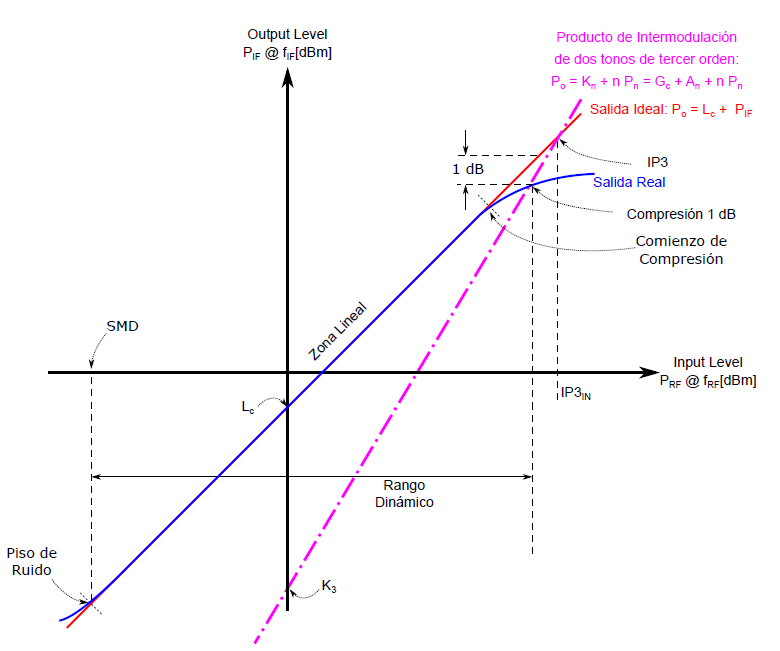
\includegraphics[width=0.8\linewidth]{imagenes/mixer}
		\caption[Relación potencia de entrada vs salida (Fuente: EA3\_mixer2025)]{Relación potencia de entrada vs salida (Fuente: EA3\_mixer2025)}
		\label{fig:mixer}
	\end{figure}
	
	El Nivel de Mezclador ($Level N$) es la potencia en dBm requerida en el puerto del Oscilador Local (LO) especificada por el fabricante para garantizar la conmutación óptima de los diodos y lograr la mínima pérdida de conversión. 
	
	\begin{table}
		\centering
		\footnotesize % Tamaño ideal para tablas extensas con 5 columnas
		\setlength{\tabcolsep}{3.5pt} % Margen lateral interno optimizado
		\renewcommand{\arraystretch}{1.25} % Altura confortable entre filas
		
		% 5 columnas X con pesos proporcionales (Suma = 0.85 + 0.75 + 1.10 + 1.15 + 1.15 = 5.0)
		\begin{tabularx}{\textwidth}{|
				>{\hsize=0.85\hsize\RaggedRight\arraybackslash}X|
				>{\hsize=0.75\hsize\RaggedRight\arraybackslash}X|
				>{\hsize=1.10\hsize\RaggedRight\arraybackslash}X|
				>{\hsize=1.15\hsize\RaggedRight\arraybackslash}X|
				>{\hsize=1.15\hsize\RaggedRight\arraybackslash}X|}
			\hline
			\textbf{Topología} & \textbf{Configuración de Dispositivos} & \textbf{Ventajas Principales} & \textbf{Desventajas / Limitaciones} & \textbf{Aplicación Típica en Satélites / RF} \\
			\hline
			\textbf{Single-Ended} \newline (Terminación Única) & 1 elemento no lineal (diodo o transistor). & Máxima simplicidad circuital y muy bajo costo de fabricación. & Nulo aislamiento entre puertos; fuga directa de $f_{LO}$ a $f_{RF}$ e $f_{IF}$; alta generación de espurias. & Detectores de RF simples, receptores de bajo costo o etapas de muy baja frecuencia. \\
			\hline
			\textbf{Singly Balanced} \newline (Simplemente Balanceado) & 2 elementos no lineales acoplados mediante un híbrido de $90^\circ$ o $180^\circ$ (balun). & Cancela armónicos pares del $LO$ o $RF$; mejora el aislamiento $LO$-$RF$ o $LO$-$IF$ ($> 20$ dB). & Requiere transformador/balun que ocupa área de sustrato; exige mayor potencia $P_{LO}$. & Receptores de microondas de complejidad moderada y sistemas terrestres. \\
			\hline
			\textbf{Double Balanced} \newline (Doblemente Balanceado) & 4 diodos en Anillo/Estrella + 2 transformadores balun ($RF$ y $LO$). & Excelente aislamiento entre todos los puertos ($> 30$--$40$ dB); rechaza productos espurios de orden par ($m f_{RF} \pm n f_{LO}$). & Mayor pérdida de inserción en baluns; requiere alta potencia de oscilador local ($P_{LO} \ge +7$ dBm). & Cargas útiles satelitales (\textit{bent-pipe}), bloques LNB y convertidores de alta linealidad. \\
			\hline
			\textbf{Subharmó-} \newline \textbf{nicamente} \newline \textbf{Balanceado} & Múltiples diodos en configuración antiparalelo excitados a $f_{LO}/2$ o $f_{LO}/n$. & Permite operar a frecuencias milimétricas ($f_{RF} > 30$ GHz) utilizando un $LO$ de menor frecuencia. & Mayor pérdida de conversión y mayor complejidad en la red de acoplamiento de entrada. & Receptores satelitales de alta frecuencia (Bandas Ka, Q/V y EHF) y enlaces intersatelitales. \\
			\hline
			\textbf{Celda de Gilbert} \newline (Activo) & Cuadripolo diferencial de 6 transistores acoplados en fuente/emisor común. & Integración monolítica (MMIC/CMOS/SiGe); provee ganancia de conversión ($G_c > 0$ dB) con bajo $P_{LO}$. & Mayor figura de ruido ($NF$); menor linealidad ($IP3$ reducido); requiere alimentación constante en DC. & Cargas útiles regenerativas (procesamiento a bordo), módems satelitales e ICs integrados. \\
			\hline
		\end{tabularx}
		
		\vspace{6pt}
		\caption{Cuadro Comparativo de Topologías de Mezcladores (Fuente: Maral, G., Bousquet, M., Z. Satellite Communications Systems)}
		\label{tab:topologias_mezcladores}
	\end{table}
	
	\subsection{Oscilador local (LO) mediante PLL}
	Un Oscilador Local (LO) es un generador de una señal senoidal de radiofrecuencia de alta pureza espectral, cuyo propósito principal es servir como señal de referencia para la conversión de frecuencia (mezcla/heterodinaje) en transmisores y receptores de RF. En la literatura clásica de telecomunicaciones, las principales tecnologías para la implementación de un LO se clasifican según su arquitectura:
	\begin{itemize}
		\item \textbf{Osciladores LC y a Cristal Libres}: Ofrecen un bajo ruido de fase pero presentan una baja estabilidad en frecuencia ante variaciones de temperatura y envejecimiento. Además, su ajuste de frecuencia es limitado o nulo.
		
		\item \textbf{DDS (Direct Digital Synthesis)}: Genera señales mediante el procesamiento numérico de muestras en el dominio del tiempo y un conversor D/A. Posee un tiempo de conmutación extremadamente rápido y alta resolución, pero está limitado en frecuencia máxima de operación y presenta un nivel elevado de espurias distantes.
		
		\item \textbf{Osciladores Sintonizados por YIG (Yttrium Iron Garnet)}: Ofrecen rangos de sintonía ultra-amplios y un ruido de fase excepcionalmente bajo, pero son volumétricamente grandes, costosos y de consumo elevado.
		
		\item \textbf{Sintetizadores por Lazo de Enganche de Fase (PLL - Phase-Locked Loop)}: Combinan la estabilidad en frecuencia de una referencia cristalina de baja frecuencia con la capacidad de generar altas frecuencias mediante un Oscilador Controlado por Voltaje (VCO). Es el estándar de la industria moderna por su equilibrio entre integrabilidad, amplio rango de sintonía y costo.
	\end{itemize}
	
	Un lazo de enganche de fase (PLL) es un sistema de realimentación que combina un oscilador controlado por voltaje (VCO) y un comparador de fase conectados de tal manera que el oscilador mantiene un ángulo de fase constante con respecto a una señal de referencia. Los lazos de enganche de fase se pueden utilizar, por ejemplo, para generar señales de salida estables de alta frecuencia a partir de una señal fija de baja frecuencia. El PLL se puede analizar como un sistema de realimentación negativa utilizando la teoría de la Transformada de Laplace con un término de ganancia directa, $G(s)$, y un término de realimentación, $H(s)$.
	
	\begin{figure}[h!]
		\centering
		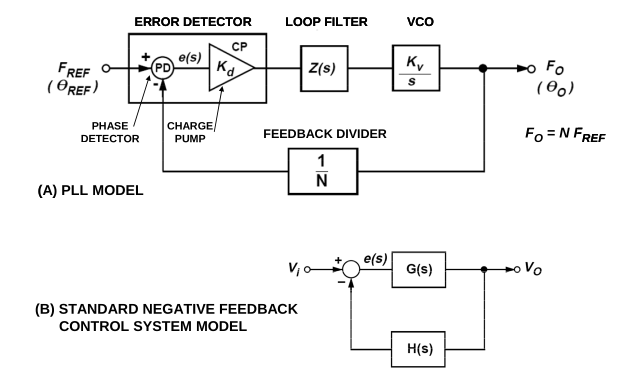
\includegraphics[width=0.7\linewidth]{imagenes/pll_1}
		\caption[Modelo basico de PLL (Fuente: MT\_086 Fundamentals PLL's)]{Modelo basico de PLL (Fuente: MT\_086 Fundamentals PLL's)}
		\label{fig:pll1}
	\end{figure}
	
	Los bloques básicos del PLL son el Detector de Error (compuesto por un detector de fase/frecuencia y una bomba de carga), el Filtro de Lazo, el VCO y un Divisor de Realimentación. La realimentación negativa fuerza a que la señal de error, $e(s)$, se aproxime a cero, punto en el cual la salida del divisor de realimentación y la frecuencia de referencia quedan enganchadas en fase y frecuencia:
	
	\begin{equation}
		F_O = N F_{REF} 
	\end{equation}
	
	En un sistema que utiliza un PLL para generar frecuencias más altas que la de entrada, el VCO oscila a una frecuencia angular $\omega_O$. Una porción de esta señal se realimenta hacia el detector de error a través de un divisor de frecuencia con una relación $1/N$. Esta frecuencia dividida se aplica a una de las entradas del detector de error. La otra entrada, en este ejemplo, es una señal de referencia fija. El detector de error compara las señales en ambas entradas. Cuando las dos señales de entrada son iguales en fase y frecuencia, el error será constante y se dice que el lazo está en condición de enganche (locked). 
	
	Una implementación habitual de un Detector de Fase/Frecuencia (PFD), que consiste básicamente en dos flip-flops tipo D. Una salida Q activa una fuente de corriente positiva y la otra salida Q activa una fuente de corriente negativa. Asumiendo que, en este diseño, los flip-flops tipo D se disparan por flanco de subida (positivo), los estados posibles se muestran en la tabla lógica.
	
	\begin{figure}[h!]
		\centering
		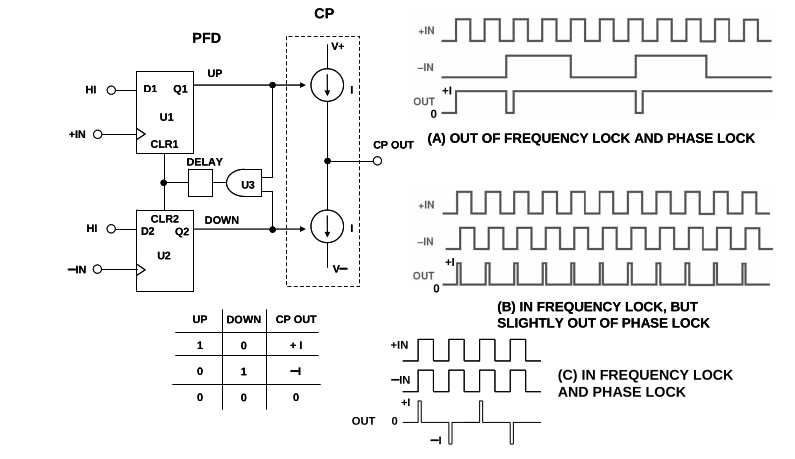
\includegraphics[width=1\linewidth]{imagenes/pll_2}
		\caption[Implementación de PFD (Fuente: MT\_086 Fundamentals PLL's)]{Implementación de PFD (Fuente: MT\_086 Fundamentals PLL's)}
		\label{fig:pll2}
	\end{figure}
	
	Si el sistema está fuera de enganche y la frecuencia en +IN es mucho mayor que la frecuencia en –IN, como se muestra en la Figura A. Dado que la frecuencia en +IN es mucho mayor que en –IN, la salida UP pasa la mayor parte del tiempo en estado alto. El primer flanco de subida en +IN lleva la salida a nivel alto y esto se mantiene hasta que se produce el primer flanco de subida en –IN. En un sistema práctico, esto significa que la salida, y por lo tanto la entrada al VCO, se lleva a un nivel más alto, lo que resulta en un aumento de la frecuencia en –IN. Esto es exactamente lo que se desea. Si la frecuencia en +IN fuera mucho menor que en –IN, ocurriría el efecto opuesto. La salida en OUT pasaría la mayor parte del tiempo en estado bajo. Esto tendría el efecto de llevar al VCO en dirección negativa y, de nuevo, acercar mucho más la frecuencia en –IN a la de +IN, para aproximarse a la condición de enganche. La Figura B muestra las formas de onda cuando las entradas están enganchadas en frecuencia y cerca del enganche de fase. Dado que +IN está adelantada respecto a –IN, la salida es una serie de pulsos de corriente positiva. Estos pulsos tenderán a controlar el VCO de modo que la señal en –IN se alinee en fase con la de +IN. Cuando esto ocurre, si no hubiera un elemento de retardo entre U3 y las entradas CLR de U1 y U2, sería posible que la salida estuviera en modo de alta impedancia, sin producir pulsos de corriente ni positivos ni negativos.\newline
	
	El VCO derivaría hasta que se desarrollara un error de fase significativo y comenzara a producir nuevamente pulsos de corriente positivos o negativos. A lo largo de un período de tiempo relativamente largo, el efecto de este ciclo sería que la salida de la bomba de carga quedaría modulada por una señal que es un subarmónico de la frecuencia de referencia de entrada del PFD. Al tratarse de una señal que puede ser de baja frecuencia, no sería atenuada por el filtro de lazo y daría lugar a espurias muy significativas en el espectro de salida del VCO, un fenómeno conocido como efecto de backlash (holgura) o "zona muerta".
	
	El elemento de retardo entre la salida de U3 y las entradas CLR de U1 y U2 garantiza que esto no suceda. Con el elemento de retardo, incluso cuando +IN y –IN están perfectamente alineadas en fase, se seguirá generando un pulso de corriente en la salida de la bomba de carga, como se muestra en la Figura C. La duración de este retardo es igual al retardo insertado en la salida de U3 y se conoce como el ancho de pulso anti-backlash.\newline
	
	El contador N, también conocido como divisor N, es el elemento programable que establece la relación entre las frecuencias de entrada y salida en el PLL. La complejidad del contador N ha aumentado con los años. Además de un contador N directo, ha evolucionado para incluir un prescaler (predivisor), el cual puede poseer un módulo doble (dual modulus). Esta estructura se desarrolló como solución a los problemas inherentes al uso de la estructura básica de división por N en el camino de realimentación hacia el detector de fase cuando se requieren frecuencias de salida muy altas. Para manejar este rango, resulta lógico anteponer al contador programable un elemento contador fijo para reducir la frecuencia de entrada alta a un rango en el que la tecnología CMOS estándar pueda trabajar. Este contador, denominado prescaler.\newline
	
	\begin{figure}[h!]
		\centering
		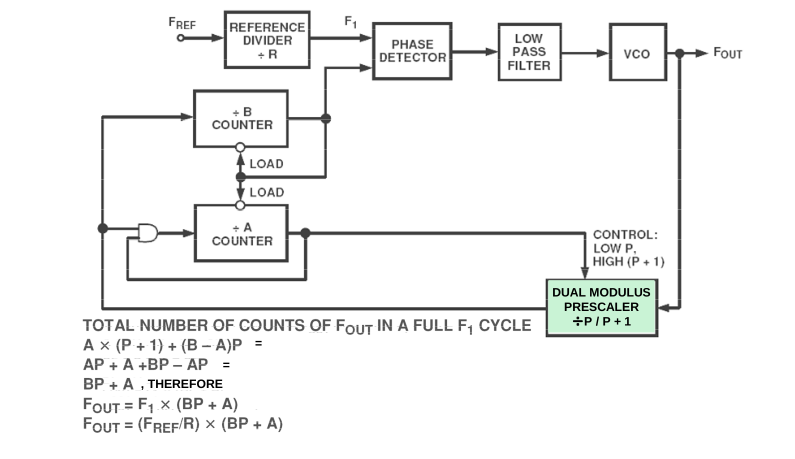
\includegraphics[width=0.75\linewidth]{imagenes/pll_3}
		\caption[Divisor entero N (Fuente: Fuente: MT\_086 Fundamentals PLL's)]{Divisor entero N (Fuente: Fuente: MT\_086 Fundamentals PLL's)}
		\label{fig:pll3}
	\end{figure}
	
	Existen múltiples especificaciones a considerar al diseñar un PLL. El rango de frecuencia RF de entrada y el espaciado de canales determinan los valores de los contadores R y N, así como los parámetros del prescaler.  El ancho de banda del lazo determina el tiempo de enganche en frecuencia y fase. Dado que el PLL es un sistema de control con realimentación negativa, se deben analizar el margen de fase y los criterios de estabilidad.  La pureza espectral de la salida del PLL se especifica mediante el ruido de fase y el nivel de las espurias relacionadas con la frecuencia de referencia.  Muchos de estos parámetros están interrelacionados; por ejemplo, anchos de banda de lazo más estrechos conducen a menores niveles de ruido de fase y espurias de referencia, pero a expensas de tiempos de enganche más lentos y un menor margen de fase.
	
	Un PLL es un tipo de oscilador y, en el diseño de cualquier oscilador, la estabilidad de frecuencia es de importancia crítica. Nos interesan tanto la estabilidad a largo plazo como la estabilidad a corto plazo. La estabilidad de frecuencia a largo plazo se refiere a cómo varía la señal de salida durante un período prolongado (horas, días o meses). Por lo general, se especifica como la relación $\Delta f/f$ para un período de tiempo determinado, expresada como un porcentaje o en dB.Por otro lado, la estabilidad a corto plazo se enfoca en las variaciones que ocurren en un período de segundos o menos. Estas variaciones pueden ser aleatorias o periódicas. Se puede utilizar un analizador de espectro para examinar la estabilidad a corto plazo de una señal.
	
	\begin{figure}[ht!]
		\centering
		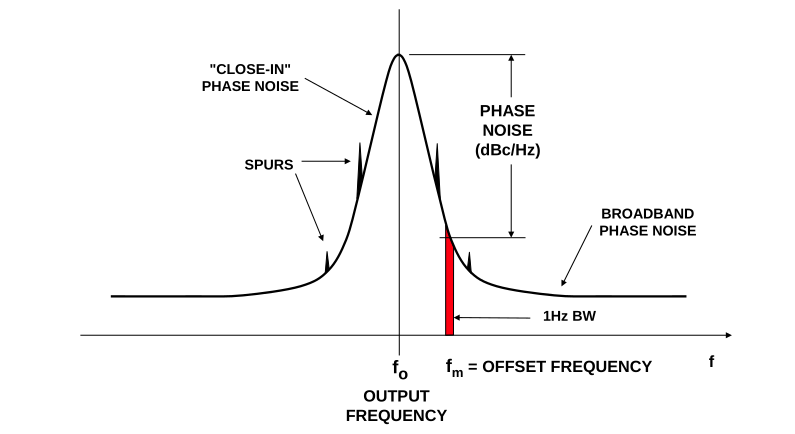
\includegraphics[width=0.8\linewidth]{imagenes/pll_4}
		\caption[Ruido de fase y componentes espurias (Fuente: Fuente: MT\_086 Fundamentals PLL's)]{Ruido de fase y componentes espurias(Fuente: Fuente: MT\_086 Fundamentals PLL's)}
		\label{fig:pll4}
	\end{figure}
	
	% ==========================================
	% MARCO METODOLÓGICO
	% ==========================================
	\part{MARCO METODOLÓGICO}
	\chapter{Requerimientos funcionales y especificaciones}
	Los requerimientos funcionales impuestos por la cátedra son los siguientes:
	
	\begin{table}[htbp]
		\centering
		\label{tab:requerimientos_rx}
		\begin{tabular}{ll}
			\toprule
			\textbf{Parámetro} & \textbf{Requerimiento / Especificación} \\
			\midrule
			Banda de recepción & 144 -- 148 MHz \\
			Ancho de banda & 80 a 100 kHz \\
			Sensibilidad & $-110$ dBm a $-95$ dBm \\
			Ganancia & $80$ dB \\
			Potencia & $< 2$ W \\
			Tensión de alimentación & 3.3 V o 5 V (a verificar conveniencia) \\
			\bottomrule
		\end{tabular}
		\caption{Requerimientos de la etapa de recepción.}
	\end{table}
	
	Adicionalmente, se impone una serie de restricciones dadas por los estándares CubeSat y PC-104. Es importante considerar que muchas de estas limitaciones no tienen una incidencia directa sobre el transpondedor, al tratarse de un subsistema específico del satélite. Asimismo, dado que la misión no está concebida para ser lanzada desde un dispensador, se omiten la mayoría de las exigencias mecánicas de despliegue. A continuación, se enumeran las especificaciones que sí resultan aplicables al diseño.
	\begin{itemize}
	\item La PCB debe responder estrictamente a las dimensiones de $90mm \times 96mm$, respetando la posición normalizada de los 4 orificios de montaje de las esquinas y la ubicación del conector de bus.
	
	\item En el apilamiento de módulos mediante espaciadores PC-104 (típicamente $15.24mm$ de separación entre placas), la altura de los componentes está restringida. Componentes voluminosos como conectores de radiofrecuencia (SMA), blindajes metálicos e inductores deben elegirse para no interferir con la placa adyacente.
	
    \item La ubicación de los componentes más pesados sobre la PCB (cajas de blindaje de RF, inductores de potencia, conectores) afecta directamente la posición final del centro de gravedad del CubeSat.
    
    \item El estándar exige un mínimo de tres inhibidores independientes para evitar cualquier emisión involuntaria de radiofrecuencia. En el diseño de la placa, esto requiere implementar físicamente tres cortes independientes en la cadena de transmisión/RF. 
    
    \item La PCB debe rutear la alimentación desde las líneas del bus central e integrar la protección adecuada contra sobrecorrientes antes de alimentar los bloques analógicos y de RF.
    
    \item Afecta la selección de materiales de fabricación de la PCB, la máscara de soldadura, la serigrafía y los recubrimientos conformados. Todos deben cumplir con $TML \le 1.0\%$ y $CVCM \le 0.1\%$.
    
    \item En el entorno espacial no existe la convección de aire. El trazado de la PCB debe incluir planos de masa continuos y vías térmicas bajo el LNA, mezcladores y reguladores para disipar el calor por conducción hacia la estructura.
    
    \item Restringe la utilización de blindajes o inductores con núcleo ferromagnético a componentes que no excedan un campo de $0.5$ Gauss sobre el campo magnético terrestre.
    
    \item La placa debe contar con circuitería o integrar señales de control desde el microcontrolador que garanticen que la RF no transmita antes de transcurrir los 45 minutos posteriores al despliegue.
    
    \item Filtrado estricto en la etapa final de salida de RF (pasa-banda/pasa-bajo) para cumplir con las reglamentaciones de emisiones fuera de banda (ENACOM, IARU, FCC) y separación de planos de masa analógicos, digitales y de RF.
	\end{itemize}
	
	Cabe destacar que, al tratarse de un proyecto con fines académicos, no resulta indispensable satisfacer al 100\% las normativas. Cumplir con todos los requerimientos impuestos por la norma maximiza la posibilidad de oportunidades de lanzamiento con los proveedores. No obstante, las especificaciones analizadas en el marco teórico representan las condiciones más restrictivas de los estándares vigentes.
	
	\chapter{Selección de componentes, diseño y simulación de los bloques funcionales} 
	
	\section{Amplificador de bajo ruido (LNA)}
	Como se explico en el marco teórico, es necesario un amplificador de bajo ruido capaz de enmascarar la figura de ruido del transponder. Los criterios para seleccionar el componentes fueron: bajo consumo de corriente, baja figura de ruido, ancho de banda que comprenda las frecuencias VHF, amplitud térmica, costo, vida útil y disponibilidad. Con todo lo anteriormente mencionado, se selecciono en PSA-5454+ de minicircuit.
	\begin{table}[htbp]
		\centering
		\label{tab:psa5454_caracteristicas}
		\begin{tabular}{|l|l|}
			\hline
			\multicolumn{2}{|c|}{\textbf{Características Principales / Desempeño (a 1 GHz)}} \\
			\hline
			Figura de ruido (\textit{Noise Figure}) & 0.8 dB (Típ.) \\
			Punto de intercepción de 3.er orden de salida (OIP3) & +25.3 dBm (Típ.) \\
			Ganancia & 18 dB (Típ.) \\
			Potencia de salida a 1 dB de compresión (Output P1dB) & +15 dBm (Típ.) \\
			Tensión de alimentación & +5 V (Alimentación única positiva) \\
			Corriente de operación ($I_D$) & 20 mA \\
			Encapsulado & SOT-363 (Tamaño microminiatura) \\
			Lavable en agua (\textit{Aqueous Washable}) & Sí \\
			\hline
			\multicolumn{2}{|c|}{\textbf{Valores Máximos Absolutos}} \\
			\hline
			Temperatura de operación & -45 °C a +85 °C \\
			Temperatura de almacenamiento & -65 °C a +150 °C \\
			Temperatura de canal & +150 °C \\
			Tensión de CC (Pin 6) & +6 V \\
			Disipación de potencia & 390 mW \\
			Corriente de CC (Pin 6) & 60 mA \\
			Corriente de polarización (Pin 4) & 10 mA \\
			Potencia de entrada (CW) & +15 dBm \\
			\hline
		\end{tabular}
		\caption{Especificaciones y valores máximos absolutos del amplificador PSA-5454+.}
	\end{table}
	
	Nota en la hoja de datos: La combinación de bajo ruido y un alto valor de OIP3 hace que este amplificador MMIC sea ideal para etapas de entrada de receptor (RFE) de bajo ruido, ya que ofrece ventajas en ambos extremos del rango dinámico: sensibilidad y rango dinámico libre de espúreas ante señales de dos tonos.\newpage
	
	\begin{figure}[h!]
		\centering
		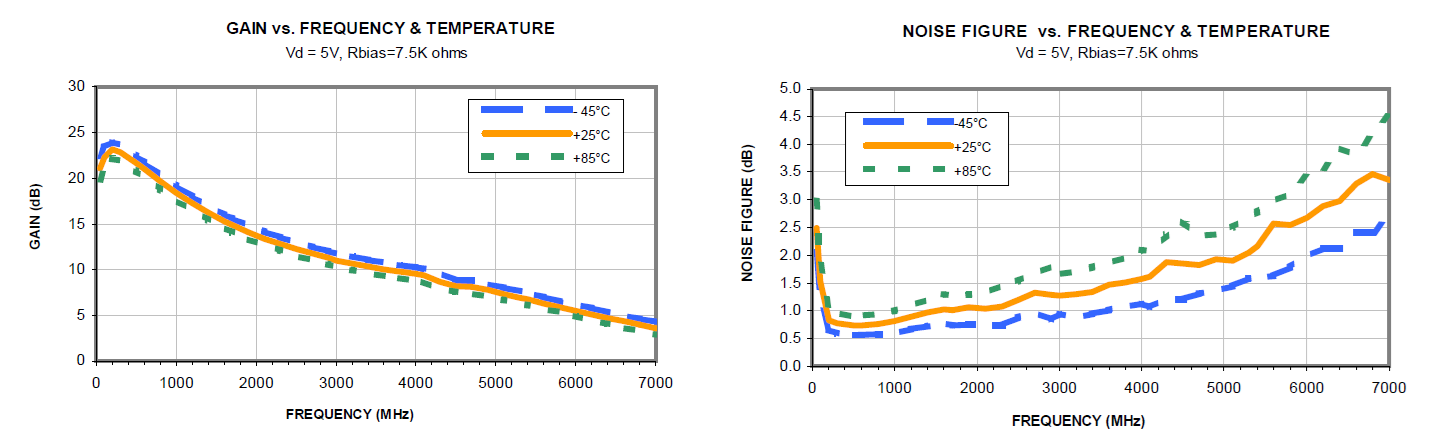
\includegraphics[width=1\linewidth]{imagenes/p_lna_1}
		\caption[Ganancia/Figura de ruido vs frecuencia (Fuente: Hoja de datos PSA-5454+ Minicircuit)]{Ganancia/Figura de ruido vs frecuencia (Fuente: Hoja de datos PSA-5454+ Minicircuit)}
		\label{fig:plna1}
	\end{figure}
	
	\begin{figure}[h!]
		\centering
		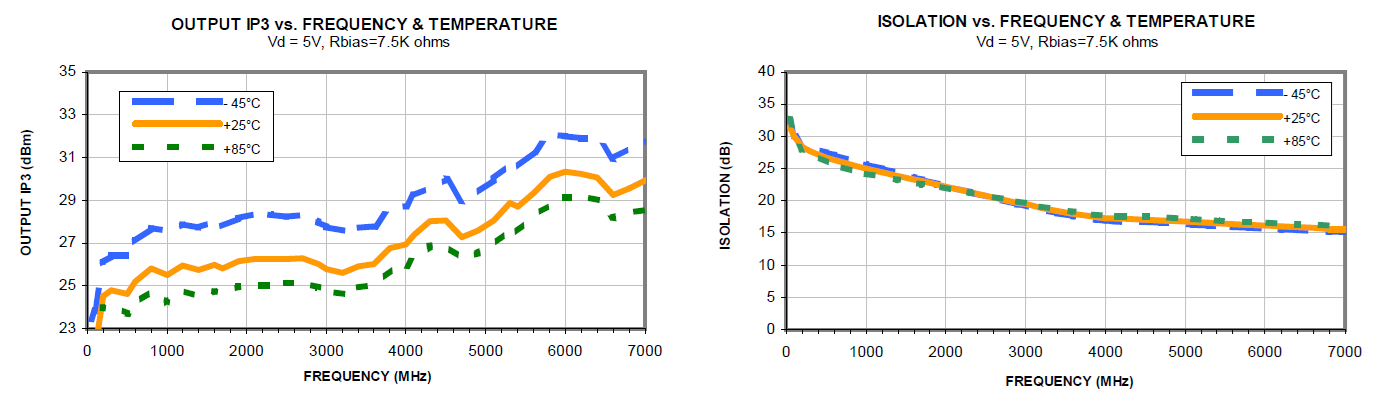
\includegraphics[width=1\linewidth]{imagenes/p_lna_2}
		\caption[IP3/Aislación inversa vs frecuencia (Fuente: Hoja de datos PSA-5454+ Minicircuit)]{IP3/Aislación inversa vs frecuencia (Fuente: Hoja de datos PSA-5454+ Minicircuit)]}
		\label{fig:plna2}
	\end{figure}
	
	Para el diseño se tuvo en cuenta el circuito recomendado por el fabricante, ya que cumple con los criterios antes mencionados y ademas se proporciona la caracterización en parámetros distribuidos (.s2p) útiles en la simulaciones.
	
	\begin{figure}[h!]
		\centering
		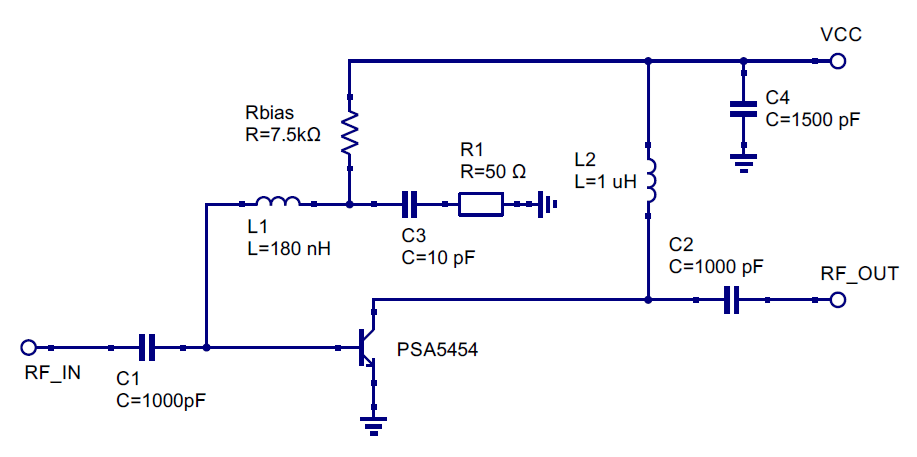
\includegraphics[width=0.8\linewidth]{imagenes/p_lna_3}
		\caption[Ciruito recomendado TEST CONDITIONS: Vd = 5V, Rbias=7.5K ohms, Id=20 mA @ Temperature =25degC]{Ciruito recomendado TEST CONDITIONS: Vd = 5V, Rbias=7.5K ohms, Id=20 mA @ Temperature =25degC}
		\label{fig:plna3}
	\end{figure}
	
	A continuación se muestran los resultados de la simulación, de los parámetros S a la frecuencia VHF deseada.
	\begin{figure}[h!]
		\centering
		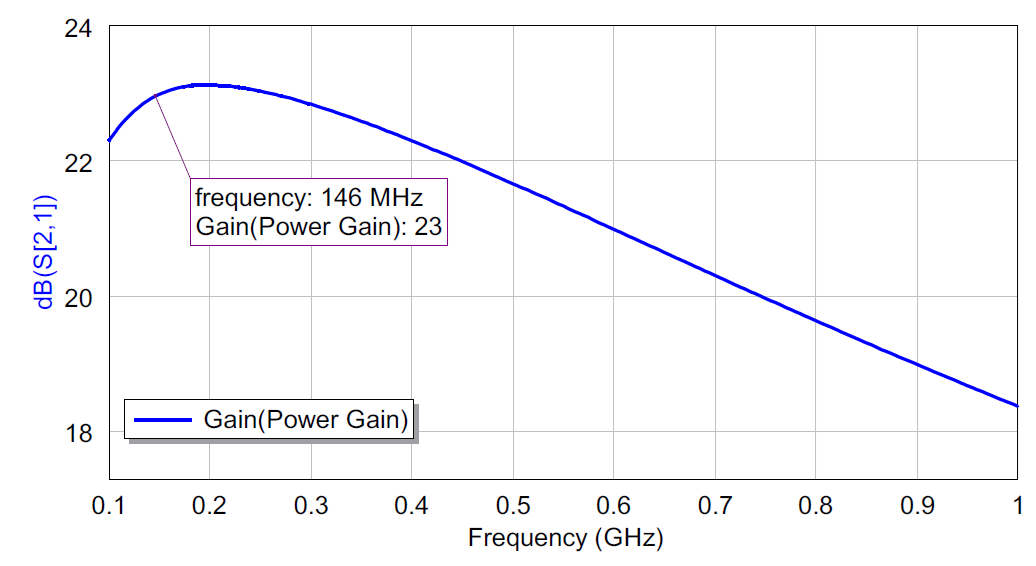
\includegraphics[width=0.8\linewidth]{imagenes/p_lna_4}
		\caption[Ganancia f=146MHz]{Ganancia f=146MHz}
		\label{fig:plna4}
	\end{figure}
	
	\begin{figure}[h!]
		\centering
		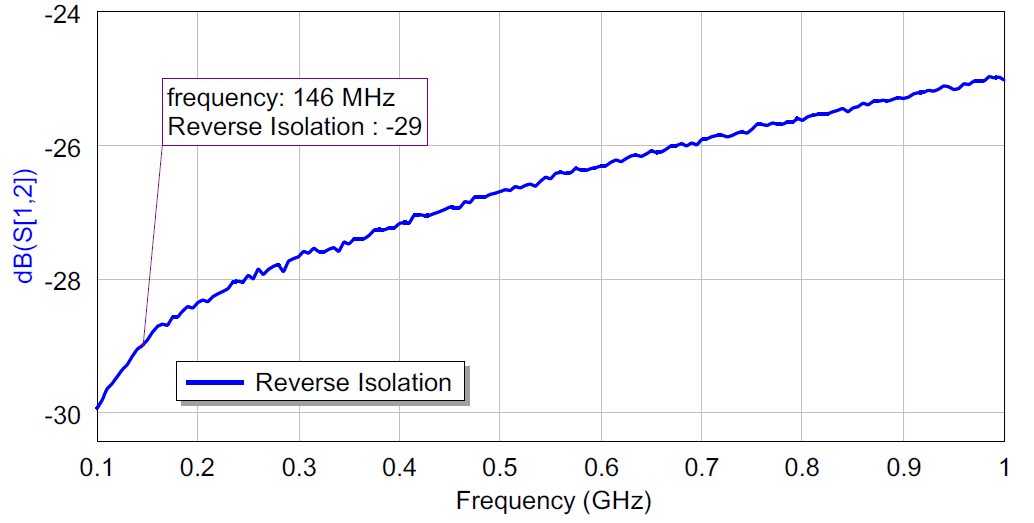
\includegraphics[width=0.8\linewidth]{imagenes/p_lna_5}
		\caption[Aislación inversa f=146MHz]{Aislación inversa f=146MHz}
		\label{fig:plna5}
	\end{figure}
	
	\begin{figure}[h!]
		\centering
		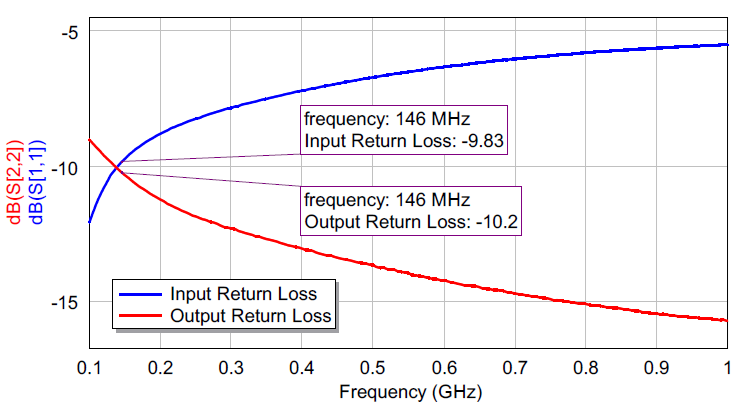
\includegraphics[width=0.85\linewidth]{imagenes/p_lna_7}
		\caption[Reflexiones directa e inversa f=146MHz]{Reflexiones directa e inversa f=146MHz}
		\label{fig:plna7}
	\end{figure}\newpage
	
	En la hoja de datos, el fabricante expone que no hace falta redes de adaptación de impedancias externas y que se encuentran adaptadas a 50 ohm. Sin embargo esto no es valido para todo el ancho de banda del amplificador (0-4HGz), por lo que resulta conveniente colocar redes de adaptación tipo T o tipo PI para mejorar los parámetros de reflexión S11 y S22. En el caso de la red de entrada, adicionalmente se debe colocar un filtro sintonizado que permita el desacople entre la entrada y la salida. 
	\begin{figure}[h!]
		\centering
		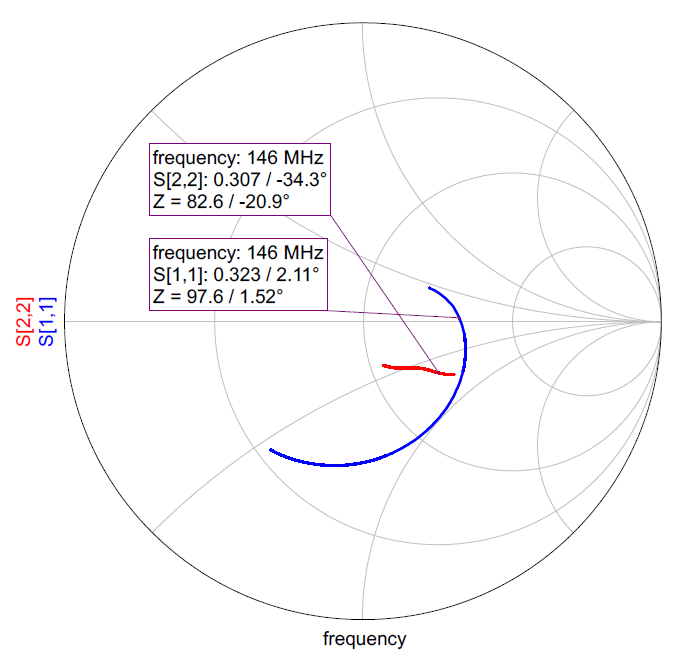
\includegraphics[width=0.7\linewidth]{imagenes/p_lna_6}
		\caption[Impedancia de entrada y salida]{Impedancia de entrada y salida}
		\label{fig:plna6}
	\end{figure}
	
	A partir de la gráfica, los parámetros S en formato polar son:
	\begin{itemize}
		\item $S_{11}$: $0.323 \angle 2.08^\circ$
		\item $S_{22}$: $0.307 \angle -34.3^\circ$
		\item $S_{21}$: $14.1 \angle 175^\circ$
		\item $S_{12}$: $0.0356 \angle 27.9^\circ$
	\end{itemize}
	
	Antes de intentar una adaptación simétrica conjugada, es obligatorio verificar si el dispositivo es incondicionalmente estable. Si no lo es, este método no se puede aplicar directamente porque ciertas impedancias harían oscilar el circuito. Calculamos el determinante ($\Delta$) y el factor de Rollett ($K$):
	\begin{equation}
		\Delta = S_{11}S_{22} - S_{12}S_{21}
	\end{equation}
	\begin{equation}
		\Delta = (0.323 \angle 2.08^\circ)(0.307 \angle -34.3^\circ) - (0.0356 \angle 27.9^\circ)(14.1 \angle 175^\circ)
	\end{equation}
	\begin{equation}
		\Delta \approx 0.546 + j0.143 = 0.565 \angle 14.6^\circ
	\end{equation}
	
	Como $\vert{}\Delta\vert{} = 0.565 < 1$, el primer criterio se cumple. Ahora calculamos $K$:
	
	\begin{equation}
		K = \frac{1 - \vert{}S_{11}\vert{}^2 - \vert{}S_{22}\vert{}^2 + \vert{}\Delta\vert{}^2}{2 \vert{}S_{12} S_{21}\vert{}}
	\end{equation}
	\begin{equation}
		K = \frac{1 - 0.323^2 - 0.307^2 + 0.565^2}{2 (0.0356 \times 14.1)}
	\end{equation}
	\begin{equation}
		K = \frac{1 - 0.104 - 0.094 + 0.319}{1.004} \approx 1.116
	\end{equation}
	
	Como $K > 1$ y $\vert{}\Delta\vert{} < 1$, el dispositivo es incondicionalmente estable a 146 MHz. Podemos proceder con la adaptación simultánea. Para encontrar los coeficientes de reflexión, se necesita calcular las variables intermedias $B_1$, $B_2$, $C_1$ y $C_2$:
	
	\begin{equation}
		B_1 = 1 + \vert{}S_{11}\vert{}^2 - \vert{}S_{22}\vert{}^2 - \vert{}\Delta\vert{}^2 = 1 + 0.104 - 0.094 - 0.319 = 0.691
	\end{equation}
	\begin{equation}
		B_2 = 1 + \vert{}S_{22}\vert{}^2 - \vert{}S_{11}\vert{}^2 - \vert{}\Delta\vert{}^2 = 1 + 0.094 - 0.104 - 0.319 = 0.671
	\end{equation}
	\begin{equation}
		C_1 = S_{11} - \Delta S_{22}^* \approx 0.209 - j0.119 = 0.241 \angle -29.7^\circ
	\end{equation}
	\begin{equation}
		C_2 = S_{22} - \Delta S_{11}^* \approx 0.076 - j0.213 = 0.226 \angle -70.4^\circ
	\end{equation}
	
	Finalmente, se aplica las fórmulas para los coeficientes de reflexión de fuente y carga. Se usa el signo negativo en el numerador para garantizar que la magnitud sea menor a 1 (lo que corresponde a impedancias pasivas reales):
	
	\begin{equation}
		\Gamma_S = \frac{B_1 - \sqrt{B_1^2 - 4\vert{}C_1\vert{}^2}}{2C_1}
	\end{equation}
	\begin{equation}
		\Gamma_S = \frac{0.691 - \sqrt{0.691^2 - 4(0.241)^2}}{2(0.241 \angle -29.7^\circ)} \approx \frac{0.195}{0.482 \angle -29.7^\circ}
	\end{equation}
	\begin{equation}
		\Gamma_S = 0.405 \angle 29.7^\circ
	\end{equation}
	
	\begin{equation}
		\Gamma_L = \frac{B_2 - \sqrt{B_2^2 - 4\vert{}C_2\vert{}^2}}{2C_2}
	\end{equation}
	\begin{equation}
		\Gamma_L = \frac{0.671 - \sqrt{0.671^2 - 4(0.226)^2}}{2(0.226 \angle -70.4^\circ)} \approx \frac{0.174}{0.452 \angle -70.4^\circ}
	\end{equation}
	\begin{equation}
		\Gamma_L = 0.385 \angle 70.4^\circ
	\end{equation}
	
	Primero, se debe convertir los coeficientes de reflexión óptimos que se calcularon previamente ($\Gamma_S$ y $\Gamma_L$) a las impedancias que el DUT necesita ver en sus terminales, utilizando la impedancia del sistema $Z_0 = 50\ \Omega$.
	
	\begin{equation}
		Z_S = Z_0 \frac{1 + \Gamma_S}{1 - \Gamma_S} = 50 \frac{1 + (0.405 \angle 29.7^\circ)}{1 - (0.405 \angle 29.7^\circ)}
	\end{equation}
	\begin{equation}
		Z_S \approx 90.75 + j43.58\ \Omega
	\end{equation}
	\begin{equation}
		Z_L = Z_0 \frac{1 + \Gamma_L}{1 - \Gamma_L} = 50 \frac{1 + (0.385 \angle 70.4^\circ)}{1 - (0.385 \angle 70.4^\circ)}
	\end{equation}
	\begin{equation}
		Z_L \approx 47.83 + j40.75\ \Omega
	\end{equation}
	
	Para la adaptación a la entrada, se utilizó una red Pi (C-L-C) pasabajos a partir de una impedancia compleja,mediante el método de la resistencia virtual ($R_v$). Este método consiste en dividir conceptualmente la red Pi en dos secciones de tipo L acopladas. Para el filtro sintonizado usamos una resistencia virtual de $15 \Omega $, esto permite obtener un factor de calidad $ Q \approx 2.5$ que determina la selectividad del filtro. En primera sección adaptará los $50 \ \Omega$ de la fuente a los $15 \ \Omega$ de nuestra resistencia virtual mediante un capacitor en derivación ($C_{in}$) y un inductor en serie ($L_1$).
	
	\begin{equation}
		Q_1 = \sqrt{\frac{R_S}{R_v} - 1} = \sqrt{\frac{50}{15} - 1} \approx 1.5275
	\end{equation}
	
	El capacitor está en paralelo con el generador, por lo que su reactancia ($X_{Cin}$) se define por:
	\begin{equation}
		X_{Cin} = \frac{R_S}{Q_1} = \frac{50}{1.5275} \approx 32.73 \ \Omega
	\end{equation}
	\begin{equation}
		C_{in} = \frac{1}{\omega \cdot X_{Cin}} = \frac{1}{(917.34 \times 10^6) \cdot 32.73} \approx 33.3 pF
	\end{equation}
	Para el inductor en serie tenemos:
	\begin{equation}
		X_{L1} = Q_1 \cdot R_v = 1.5275 \cdot 15 = 22.91 \ \Omega
	\end{equation}
	
	La segunda sección debe adaptar la resistencia virtual de $15 \ \Omega$ a la impedancia objetivo compleja $Z_{out} = 90.75 + j43.58 \ \Omega$. Para facilitar el cálculo del capacitor en derivación ($C_{out}$), resulta indispensable convertir la impedancia objetivo en serie a su equivalente en paralelo (admitancia $Y_{out}$):
	\begin{equation}
		Y_{out} = \frac{1}{Z_{out}} = \frac{1}{90.75 + j43.58}
	\end{equation}
	\begin{equation}
		Y_{out} = \frac{90.75 - j43.58}{90.75^2 + 43.58^2} = \frac{90.75 - j43.58}{10134.77}
	\end{equation}
	\begin{equation}
		Y_{out} \approx 0.008955 - j0.004300 \ S
	\end{equation}
	
	De este resultado se deduce que la impedancia objetivo equivale a una resistencia en paralelo de $R_p = \frac{1}{0.008955} \approx 111.68 \ \Omega$ y una susceptancia inductiva de $-0.004300 \ S$.
	\begin{equation}
		Q_2 = \sqrt{\frac{R_p}{R_v} - 1} = \sqrt{\frac{111.68}{15} - 1} \approx 2.5387
	\end{equation}
	\begin{equation}
		X_{L2} = Q_2 \cdot R_v = 2.5387 \cdot 15 = 38.08 \ \Omega
	\end{equation}
	
	El nodo final está compuesto por la admitancia resultante de la red ($Y_{L2}$) en paralelo con la susceptancia de $C_{out}$ ($j\omega C_{out}$). La red proveniente de $L_2$ nos entrega la siguiente admitancia:
	\begin{equation}
		Y_{L2} = \frac{1}{R_v + jX_{L2}} = \frac{1}{15 + j38.08} = 0.008955 - j0.02273 \ S
	\end{equation}
	
	Para alcanzar el objetivo final $Y_{out}$, la suma de la susceptancia de $Y_{L2}$ y del capacitor $C_{out}$ debe ser igual a la susceptancia objetivo:
	\begin{equation}
		-j0.02273 + j\omega C_{out} = -j0.004300
	\end{equation}
	
	Despejando la susceptancia del capacitor:
	\begin{equation}
		\omega C_{out} = 0.02273 - 0.004300 = 0.01843 \ S
	\end{equation}
	\begin{equation}
		C_{out} = \frac{0.01843}{\omega} = \frac{0.01843}{917.34 \times 10^6} \approx 20.09 pF
	\end{equation}
	
	Como las dos redes L están conectadas en serie a través de la resistencia virtual, los inductores $L_1$ y $L_2$ se suman para formar el componente físico único de la red Pi.
	\begin{equation}
		X_{L_{serie}} = X_{L1} + X_{L2} = 22.91 + 38.08 = 60.99 \ \Omega
	\end{equation}
	\begin{equation}
		L_{serie} = \frac{X_{L_{serie}}}{\omega} = \frac{60.99}{917.34 \times 10^6} \approx 66.48 nH
	\end{equation}
	
	Para la adaptación a la salida se tiene los $Z_S = 90.75 + j43.58\ \Omega$ (vista desde el DUT) a los $50\ \Omega$ de la carga. Calculando las reactancias necesarias para esta transformación: Reactancia del inductor $X_L = 50.94\ \Omega$, susceptancia del capacitor: $B_C = 0.00426\ S$
	\begin{equation}
		L_{out} = \frac{X_L}{2\pi f} = \frac{50.94}{2\pi (146 \times 10^6)} \approx 55.5nH
	\end{equation}
	\begin{equation}
		C_{out} = \frac{B_C}{2\pi f} = \frac{0.00426}{2\pi (146 \times 10^6)} \approx 4.64pF
	\end{equation}
	
	Lo siguiente es obtener los parámetros S del amplificador con las redes de adaptación para ver el resultado obtenido, ajustando el valor de los componentes pasivos a valores comercialmente disponibles.
	\begin{figure}[h!]
		\centering
		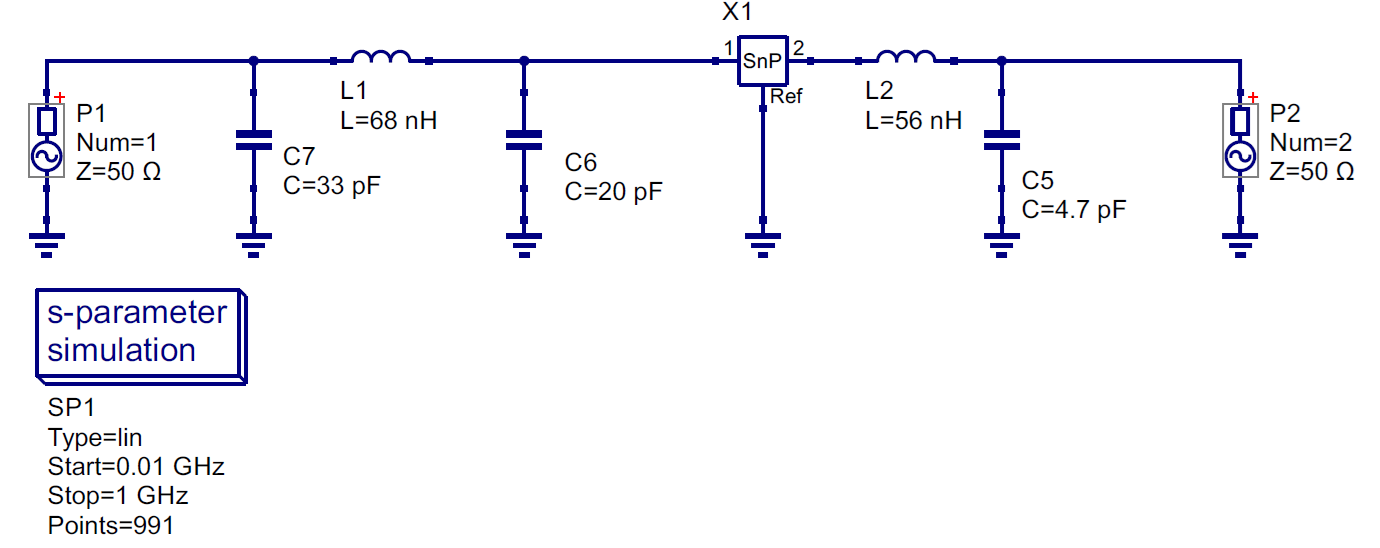
\includegraphics[width=1\linewidth]{imagenes/p_lna_12}
		\caption[Amplificador PSA-5454+ con redes de adaptación y filtro sintonizado]{Amplificador PSA-5454+ con redes de adaptacion y filtro sintonizado}
		\label{fig:plna12}
	\end{figure}
	
	\begin{figure}
		\centering
		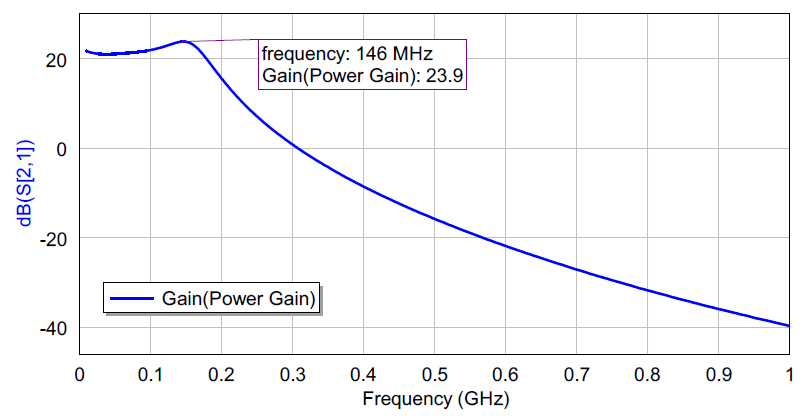
\includegraphics[width=0.8\linewidth]{imagenes/p_lna_8}
		\caption[Ganancia con filtro sintonizado]{Ganancia con filtro sintonizado}
		\label{fig:plna8}
	\end{figure}
	
	\begin{figure}
		\centering
		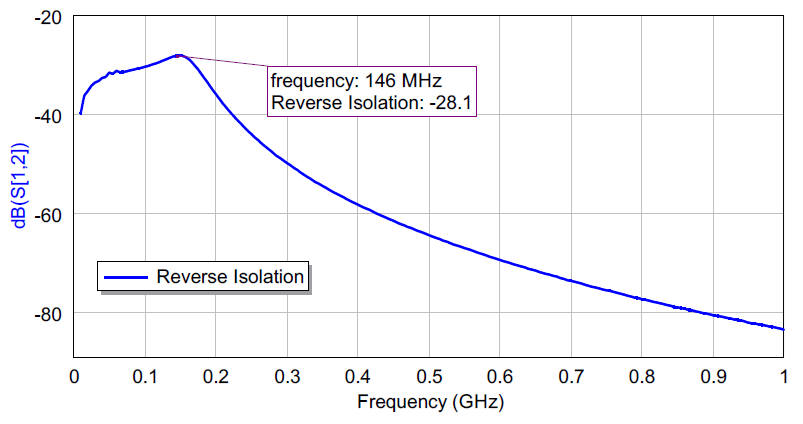
\includegraphics[width=0.8\linewidth]{imagenes/p_lna_9}
		\caption[Aislación inversa f=146MHz]{Aislación inversa f=146MHz}
		\label{fig:plna9}
	\end{figure}
	
	\begin{figure}
		\centering
		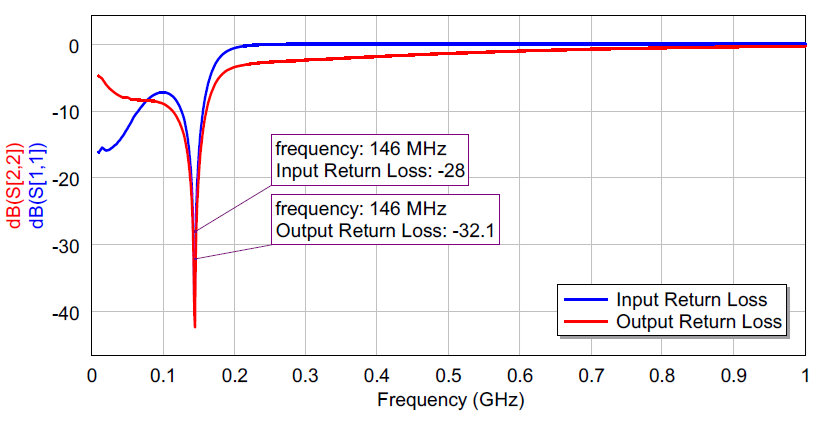
\includegraphics[width=0.8\linewidth]{imagenes/p_lna_10}
		\caption[Reflexiones directa e inversa a f=146MHz]{Reflexiones directa e inversa a f=146MHz}
		\label{fig:plna10}
	\end{figure}\newpage
	
	\begin{figure}
		\centering
		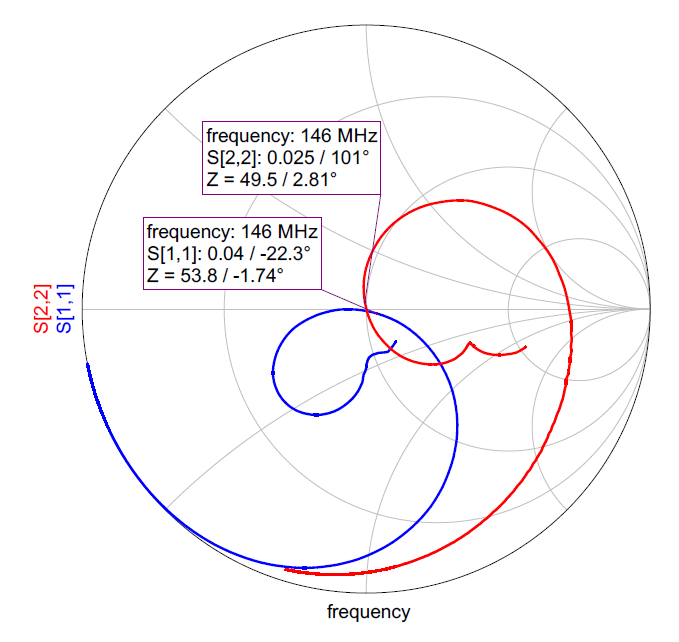
\includegraphics[width=0.7\linewidth]{imagenes/p_lna_11}
		\caption[Adaptación de impedancia a f=146MHz]{Adaptación de impedancia a f=146MHz}
		\label{fig:plna11}
	\end{figure}
	
	\section{Etapa de amplificación}
	Para cumplir con la ganancia requerida, es necesario añadir etapas de amplificación adicionales, ya que existe un limite de la cantidad de ganancia que se puede conseguir en una sola etapa. La ganancia requerida es de 80dB, teniendo en cuenta el factor de forma reducido de la PCB da como resultado una densidad de ganancia importante 17.77dB/cm aproximadamente. Bajo estas condiciones cualquier capacidad parásita existente ya sea en la PCB o en los componentes puede causar una realimentación en fase provocando la auto-oscilación del circuito volviéndolo inútil. Para mitigar estos problemas se tuvieron en cuenta las siguientes consideraciones:
	
	\begin{itemize}
			\item En primer lugar para las etapas de amplificación se seleccionó una configuración Cascode. Esta topología tiene una serie de ventajas respecto a la configuración típica de emisor común. El primero es que cancela el efecto Miller y reduce la capacidad parásita colector-base, por otro lado aumenta la aislación inversa (S12) importante para que la señal en la ultima etapa presente mas dificultades para retornar a la primer etapa.
			
			\item Otro camino por el cual la señal amplificada se puede realimentar es por medio de VCC, por lo que cada etapa esta aislada entre si con atenuadores en la linea de alimentación.
			
			\item Finalmente el ultimo camino de realimentación es por medio del aire. Para solucionar esto se coloca un blindaje en forma tabicada separando cada una de las etapas amplificadoras.
			
			\item Si con todas las precauciones anteriormente mencionadas, existiera alguna capacidad parásita que haga oscilar el circuito se colocaron pads previstos para atenuadores entre etapas para bajar la ganancia hasta donde sea necesario para estabilizarlo, y no tener que descartar el diseño.
	\end{itemize}
	
	Para el diseño se utilizo un transistor proporcionado por la cátedra (BJT 2SC3356) con las siguientes características:
	\begin{table}[htbp]
		\centering
		\label{tab:transistor_caracteristicas}
		\begin{tabular}{|l|l|}
			\hline
			\multicolumn{2}{|c|}{\textbf{Características Eléctricas ($T_A = 25\ ^\circ C$)}} \\
			\hline
			Corriente de corte de colector ($I_{CBO}$) & 1.0 $\mu$A (Máx.) \\
			Corriente de corte de emisor ($I_{EBO}$) & 1.0 $\mu$A (Máx.) \\
			Ganancia de corriente en CC ($h_{FE}$) & 120 (Típ.) [Mín. 50, Máx. 300] \\
			Producto ganancia-ancho de banda ($f_T$) & 7 GHz (Típ.) \\
			Capacidad de realimentación ($C_{re}$) & 0.55 pF (Típ.) / 1.0 pF (Máx.) \\
			Ganancia de potencia de inserción ($|S_{21e}|^2$) & 11.5 dB (Típ. a 1 GHz) \\
			Figura de ruido (\textit{Noise Figure}, $NF$) & 1.1 dB (Típ.) / 2.0 dB (Máx. a 1 GHz) \\
			\hline
			\multicolumn{2}{|c|}{\textbf{Valores Máximos Absolutos ($T_A = 25\ ^\circ C$)}} \\
			\hline
			Tensión colector-base ($V_{CBO}$) & 20 V \\
			Tensión colector-emisor ($V_{CEO}$) & 12 V \\
			Tensión emisor-base ($V_{EBO}$) & 3.0 V \\
			Corriente de colector ($I_C$) & 100 mA \\
			Disipación total de potencia ($P_T$) & 200 mW \\
			Temperatura de juntura ($T_j$) & +150 °C \\
			Temperatura de almacenamiento ($T_{stg}$) & -65 °C a +150 °C \\
			\hline
		\end{tabular}
		\caption{Características eléctricas y valores máximos absolutos del transistor 2SC3356.}
	\end{table}
	
	Para el diseño del amplificador se eligió una polarización en cadena (Ladder Biasing), ademas de un punto Q con una corriente $ICQ=10mA$ para minimizar la figura de ruido.
	\begin{figure}[h!]
		\centering
		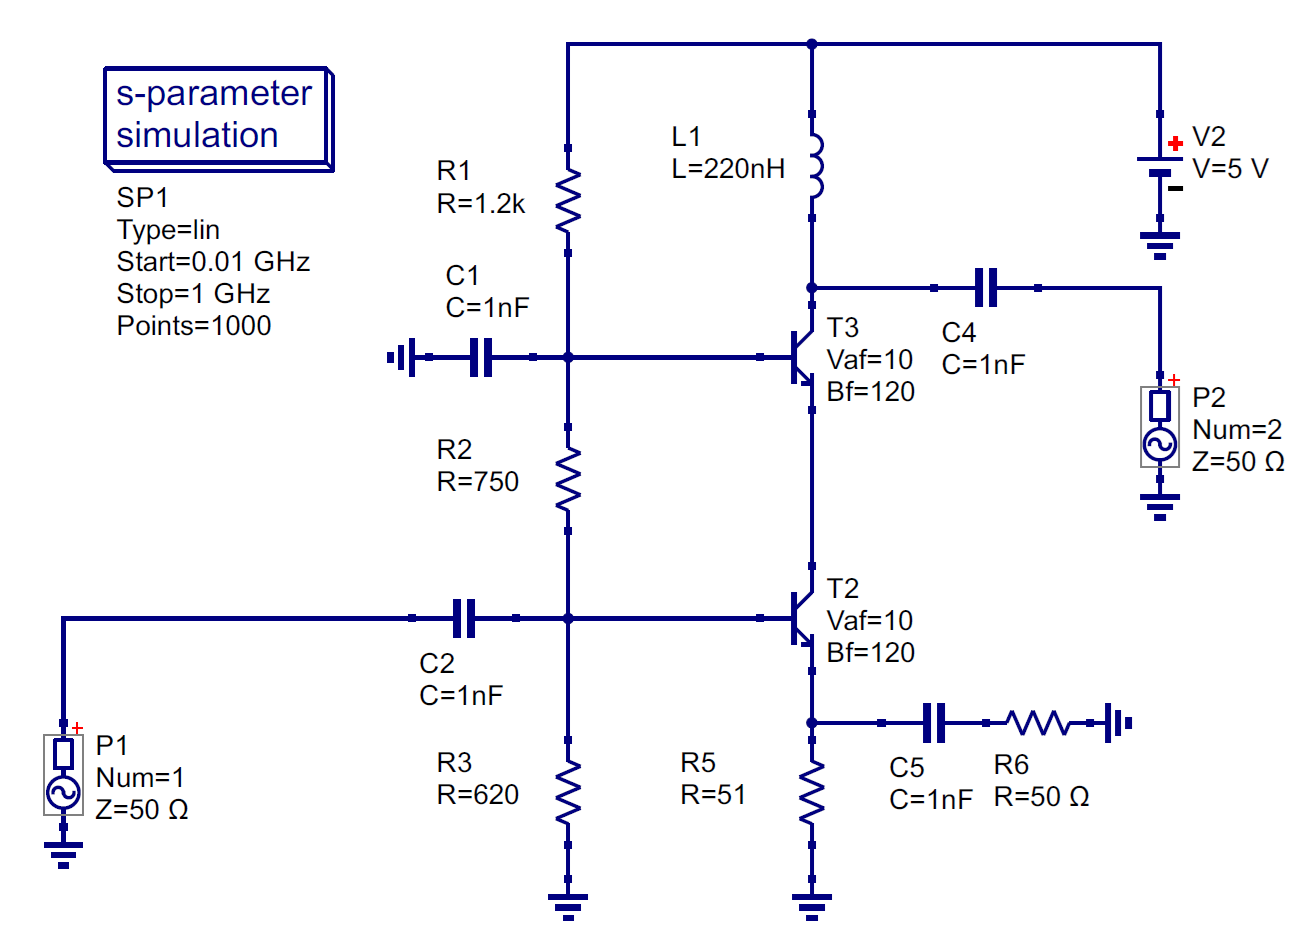
\includegraphics[width=0.7\linewidth]{imagenes/cascode_1}
		\caption[Propuesta para el amplificador Cascode]{Propuesta para el amplificador Cascode}
		\label{fig:cascode1}
	\end{figure}
	
	El primer paso en el diseño de cualquier amplificador polarizado por divisor de tensión es asegurar la estabilidad térmica. El criterio clásico de diseño establece que la tensión en la resistencia de emisor ($V_{E2}$) debe ser aproximadamente el 10\% de la tensión de alimentación ($V_{CC}$).
	\begin{equation}
		V_{E2} = 0.10 \cdot 5V = 0.5V
	\end{equation}
	Sabiendo que la corriente de emisor es prácticamente la corriente objetivo ($I_E \approx I_{CQ} = 10 mA$), calculamos $R_5$:
	\begin{equation}
		R_5 = \frac{V_{E2}}{I_{CQ}} = \frac{0.5V}{10mA} = 50 \ \Omega
	\end{equation}
	
	Para que T2 conduzca, su base debe estar $0.7V$ por encima de su emisor:
	\begin{equation}
		V_{B2} = V_{E2} + V_{BE} = 0.5V + 0.7V = 1.20V
	\end{equation}
	
	Para calcular la base de T3 ($V_{B3}$),se debe decidir cómo repartir la tensión restante para asegurar que ambos transistores operen cómodamente en la región activa lineal (evitando la saturación). Se asignó al transistor inferior (T2) una tensión colector-emisor de aproximadamente $V_{CE2} = 1.5V$ para darle un margen dinámico amplio. Sabiendo que el colector de T2 está conectado directamente al emisor de T3:
	\begin{equation}
		V_{E3} = V_{E2} + V_{CE2} = 0.5V + 1.5V = 2.0V
	\end{equation}
	
	Con esto, se define la tensión necesaria en la base del transistor superior:
	\begin{equation}
		V_{B3} = V_{E3} + V_{BE} = 2.0V + 0.7V = 2.7V
	\end{equation}
	
	Para calcular las resistencias, primero se determina la corriente de base nominal que consumirán los transistores:
	\begin{equation}
		I_B = \frac{I_{CQ}}{\beta} = \frac{10 mA}{120} \approx 83.3 \ \mu A
	\end{equation}
	
	La corriente que circula de arriba a abajo por el divisor ($I_{div}$) debe ser mucho mayor que las corrientes de base. Una regla es hacer $I_{div}$ entre 10 y 20 veces $I_B$. Se fija una corriente de divisor de $I_{div} = 2 mA$.Esta corriente $I_{div}$ es la que circulará íntegramente por la resistencia inferior ($R_3$):
	\begin{equation}
		R_3 = \frac{V_{B2}}{I_{div}} = \frac{1.2V}{2mA} = 600 \ \Omega
	\end{equation}
	
	La corriente que pasa por $R_2$ es la corriente del divisor más la corriente que se "fuga" hacia la base de T2:
	\begin{equation}
		I_{R2} = I_{div} + I_{B2} = 2.0mA + 0.083mA = 2.083mA
	\end{equation}
	
	La caída de tensión en $R_2$ es la diferencia entre ambas bases:
	\begin{equation}
		V_{R2} = V_{B3} - V_{B2} = 2.7V - 1.2V = 1.50V
	\end{equation}
	\begin{equation}
		R_2 = \frac{V_{R2}}{I_{R2}} = \frac{1.50V}{2.083 mA} = 720 \ \Omega
	\end{equation}
	
	Finalmente,el último escalón ($R_1$). La corriente que la atraviesa debe alimentar al divisor, a la base de T2 y a la base de T3:
	\begin{equation}
		I_{R1} = I_{R2} + I_{B3} = 2.083mA + 0.083mA = 2.166mA
	\end{equation}
	
	La caída de tensión en $R_1$ es la diferencia entre la fuente y la base superior:
	\begin{equation}
		V_{R1} = V_{CC} - V_{B3} = 5.0V - 2.7V = 2.3V
	\end{equation}
	\begin{equation}
		R_1 = \frac{V_{R1}}{I_{R1}} = \frac{2.3 V}{2.166 mA} \approx 1061 \ \Omega
	\end{equation}
	
	Con el diseño de la polarización, lo restante es adaptar la impedancia del amplificador a 50 $\Omega$. El resultado de las simulaciones son los siguientes.
	\begin{figure}[h!]
		\centering
		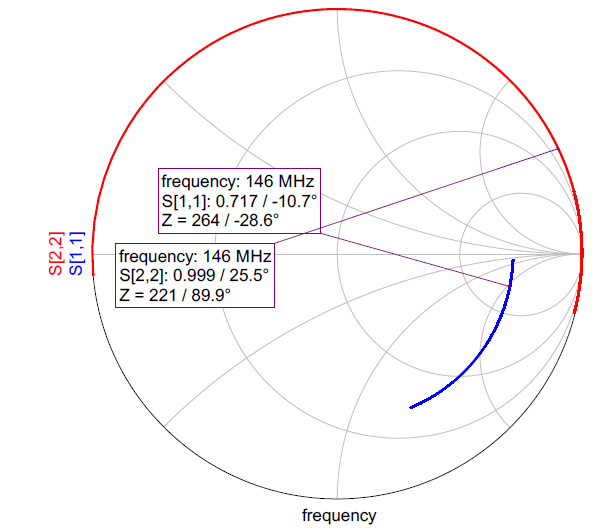
\includegraphics[width=0.7\linewidth]{imagenes/cascode_7}
		\caption[Impedancias de entrada y salida con ICQ=10mA.]{Impedancias de entrada y salida con ICQ=10mA.}
		\label{fig:cascode7}
	\end{figure}
	
	Según la simulación, la impedancia de entrada bruta del amplificador (vista desde $C_2$) es $Z_{in} = 264 \angle -28.6^\circ \ \Omega$.Para diseñar una red L, se debe pasar esta impedancia a su equivalente en paralelo (una resistencia en paralelo con un capacitor).Pasando a forma rectangular:
	\begin{equation}
		Z_{in} = 264 \cos(-28.6^\circ) + j 264 \sin(-28.6^\circ) \approx 231.8 - j126.3 \ \Omega
	\end{equation}
	
	Calculamos la admitancia ($Y_{in}$):
	\begin{equation}
		Y_{in} = \frac{1}{231.8 - j126.3} = 3.32mS + j1.81mS
	\end{equation}
	
	De aquí extraemos que el amplificador se comporta a la entrada como una resistencia $R_p$ en paralelo con un capacitor parásito $C_p$:
	\begin{equation}
		R_p = \frac{1}{3.32mS} \approx 301 \ \Omega
	\end{equation}
	\begin{equation}
		C_p = \frac{1.81mS}{2 \pi \cdot 146 MHz} \approx 1.97 pF
	\end{equation}
	
	Usamos una red "L" con un elemento paralelo del lado de alta impedancia (el transistor) y un elemento serie del lado de $50 \ \Omega$.
	\begin{equation}
		Q = \sqrt{\frac{R_p}{R_s} - 1} = \sqrt{\frac{301}{50} - 1} = \sqrt{5.02} \approx 2.24
	\end{equation}
	
	La red requiere una susceptancia inductiva para lograr la adaptación, pero además debe cancelar la susceptancia del capacitor parásito intrínseco ($1.81 mS$).
	\begin{equation}
		B_{red} = \frac{Q}{R_p} = \frac{2.24}{301} = 7.44 mS
	\end{equation}
	\begin{equation}
		B_{total} = B_{red} + B_{parásito} = 7.44mS + 1.81 mS = 9.25mS
	\end{equation}
	\begin{equation}
		X_L = \frac{1}{9.25 mS} = 108.1 \ \Omega
	\end{equation}
	\begin{equation}
		L2 = \frac{X_L}{2 \pi \cdot 146MHz} = \frac{108.1}{917 \times 10^6} \approx 117.8 nH
	\end{equation}
	
	Cálculo del capacitor serie (C3):
	\begin{equation}
		X_C = Q \cdot R_s = 2.24 \cdot 50 = 112 \ \Omega
	\end{equation}
	\begin{equation}
		C3 = \frac{1}{2 \pi \cdot 146MHz \cdot 112 \ \Omega} \approx 9.7 pF
	\end{equation}
	
	En el circuito sin adaptar, la Carta de Smith te arrojó $Z_{out} = 221 \angle 89.9^\circ \ \Omega$. Un ángulo de casi $90^\circ$ significa que el Cascode tiene una resistencia de salida colosal (decenas de kilo-ohms).Si se intentara adaptar una impedancia tan alta directamente a $50 \ \Omega$, el $Q$ sería altísimo, el ancho de banda sería microscópico y el amplificador sería inestable. Por esto el diseño adaptado añadiste $R_4 = 1k\Omega$ en paralelo. Esta resistencia es la clave: domina la impedancia de salida fijando intencionalmente $R_p = 1000 \ \Omega$ para controlar la ganancia y el ancho de banda.
	Cálculo del factor de calidad (Q) de la red:
	\begin{equation}
		Q = \sqrt{\frac{1000}{50} - 1} = \sqrt{19} \approx 4.36
	\end{equation}
	
	Cálculo del inductor de sintonía (L1):
	\begin{equation}
		X_L = \frac{R_p}{Q} = \frac{1000}{4.36} = 229.4 \ \Omega
	\end{equation}
	\begin{equation}
		L1 = \frac{229.4}{2 \pi \cdot 146MHz} \approx 250 nH
	\end{equation}
	
	Cálculo del capacitor serie (C4):
	\begin{equation}
		X_C = Q \cdot R_s = 4.36 \cdot 50 = 218 \ \Omega
	\end{equation}
	\begin{equation}
		C4 = \frac{1}{2 \pi \cdot 146MHz \cdot 218 \ \Omega} \approx 5.0pF
	\end{equation}
	
	En las siguientes simulaciones se observa que tanto los puertos de entrada como de salida están perfectamente adaptados a $50 \Omega $ ademas de proporcionar una ganancia de 19dB, junto con una aislación inversa excelente de -64dB tal como se anticipo en un principio. Resta por concatenar tres etapas Cascode junto con los atenuadores en VCC y en la red de señal, para obtener la respuesta total de la cadena de RF.
	
	\begin{figure}[h!]
		\centering
		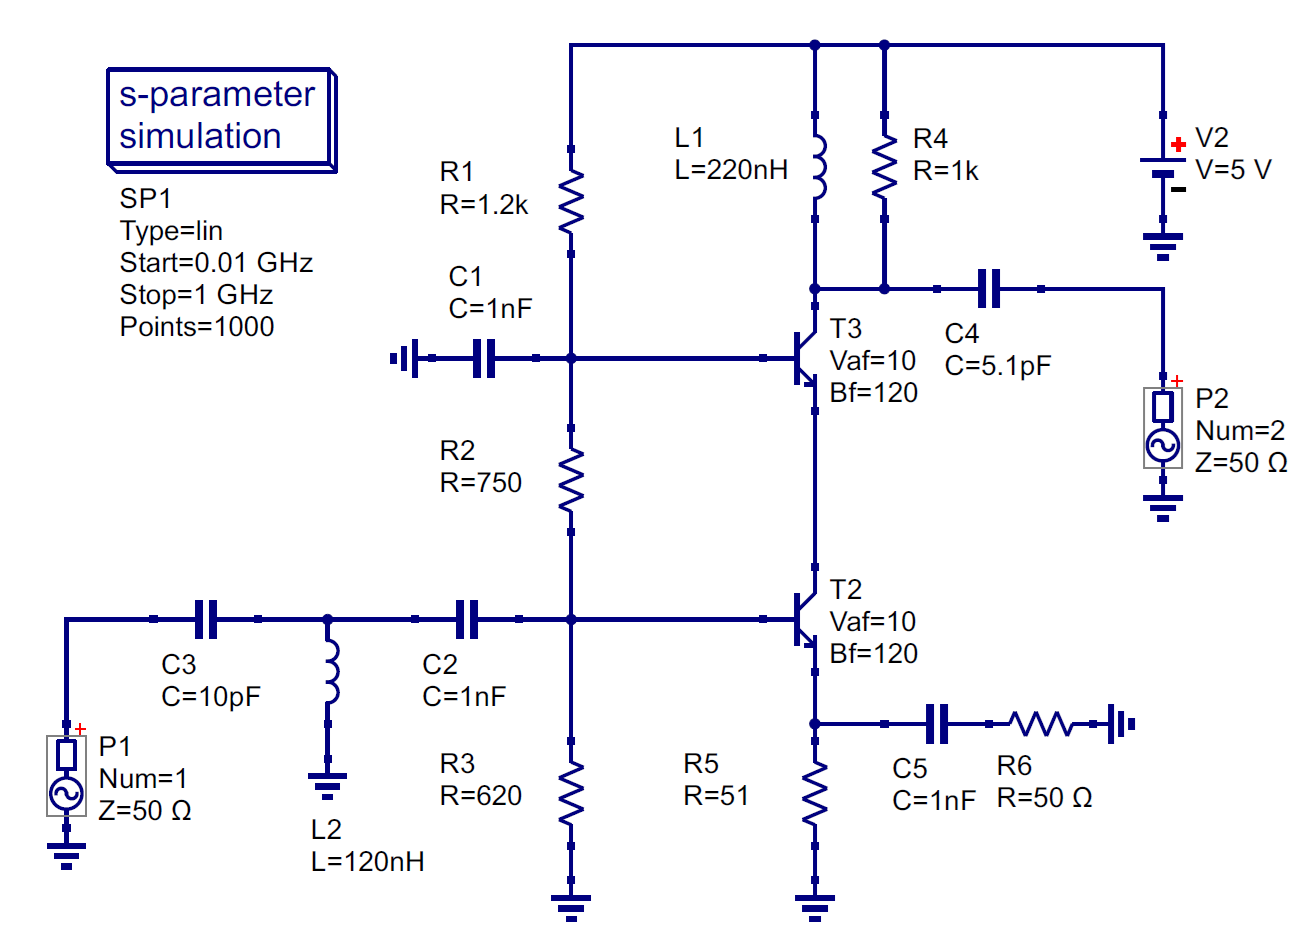
\includegraphics[width=0.7\linewidth]{imagenes/cascode_2}
		\caption[Circuito Cascode con redes de adaptación]{Circuito Cascode con redes de adaptación}
		\label{fig:cascode2}
	\end{figure}
	
	\begin{figure}[h!]
		\centering
		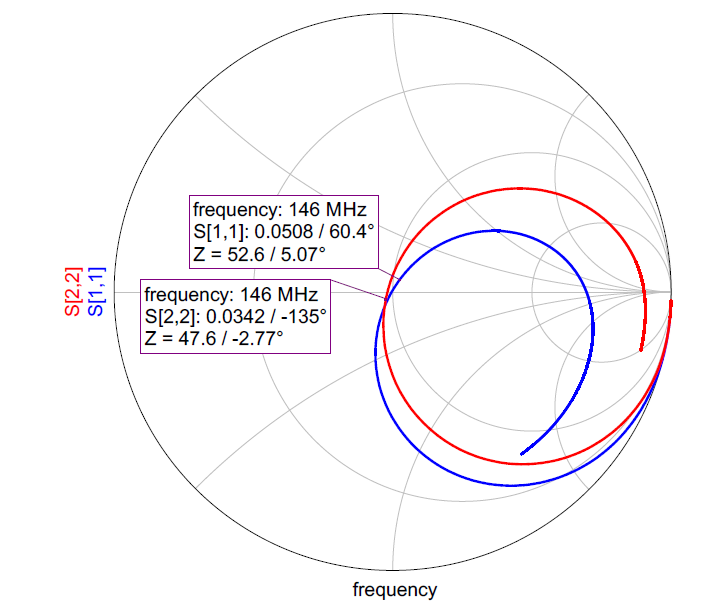
\includegraphics[width=0.75\linewidth]{imagenes/cascode_6}
		\caption[Impedancias de entrada y salida]{Impedancias de entrada y salida}
		\label{fig:cascode6}
	\end{figure}
	
	\begin{figure}[h!]
		\centering
		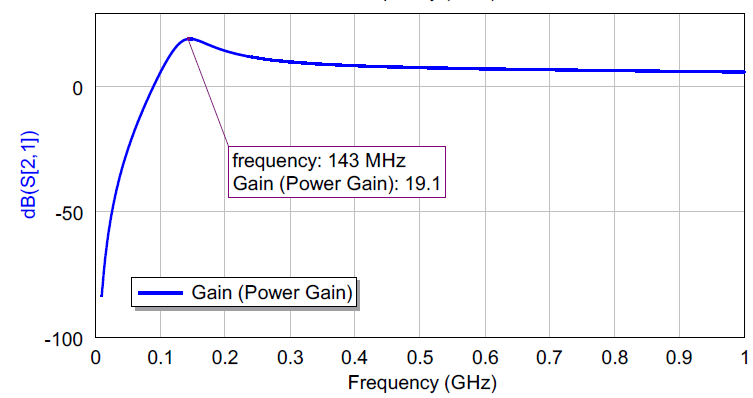
\includegraphics[width=0.8\linewidth]{imagenes/cascode_4}
		\caption[Ganancia de la etapa Cascode adaptada a 50 ohm]{Ganancia de la etapa Cascode adaptada a 50 ohm}
		\label{fig:cascode4}
	\end{figure}
	
	\begin{figure}[h!]
		\centering
		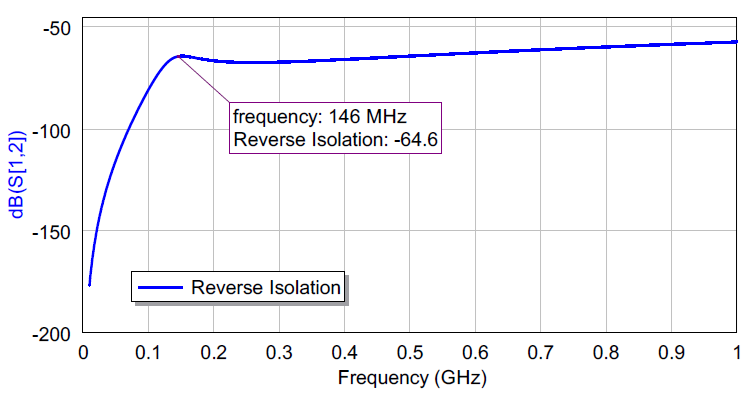
\includegraphics[width=0.8\linewidth]{imagenes/cascode_5}
		\caption[Aislación inversa de la etapa Cascode adaptada a 50 ohm]{Aislación inversa de la etapa Cascode adaptada a 50 ohm}
		\label{fig:cascode5}
	\end{figure}
	
	
	
	
	\section{Oscilador local (LO):}
	Se describe el modelo terminado, funcionalidad, manual, mediciones, etc.
	
	\section{Etapa de mezclador (Mixer)}
	Se describe el modelo terminado, funcionalidad, manual, mediciones, etc.
	
	\section{Filtro de salida}
	Se describe el modelo terminado, funcionalidad, manual, mediciones, etc.
	
	\chapter{Diseño e implementación de la placa}
	
	\section{Consideraciones de la placa para el diseño en RF}
	\section{Consideraciones de la placa para integridad de señal}
	\section{Implementación del circuito}
	
	% ==========================================
	% RESULTADOS Y CONCLUSIONES
	% ==========================================
	\part{RESULTADOS Y CONCLUSIONES}
	\chapter*{Resultados}
	\addcontentsline{toc}{chapter}{Resultados}
	(Los Resultados no deben incluirse en un Capítulo numerado, es un apartado individual).
	
	\chapter*{Conclusiones}
	\addcontentsline{toc}{chapter}{Conclusiones}
	- Resultados obtenidos en relación a la SAT. \\
	- Conclusión General. \\
	- Aporte a la Ingeniería. \\
	(Tampoco es un capítulo numerado).
	
	% ==========================================
	% BIBLIOGRAFÍA Y REFERENCIAS
	% ==========================================
	\clearpage
	\begin{spacing}{1} % Espacio simple para bibliografía
		\chapter*{Bibliografía}
		\addcontentsline{toc}{chapter}{Bibliografía}
		Aquí van SOLO libros físicos o ebooks con ISBN.
		\begin{enumerate}
			\item \setlength{\itemsep}{0.5\baselineskip} Autor. (Año). Título. Editorial. ISBN.
		\end{enumerate}
		
		\chapter*{Referencias}
		\addcontentsline{toc}{chapter}{Referencias}
		Todo lo que no son libros (Links, Inteligencia Artificial, apuntes). La numeración continúa desde la Bibliografía.
		\begin{enumerate}
			\setcounter{enumi}{1} % Continuar numeración
			\item \setlength{\itemsep}{0.5\baselineskip} OpenAI. (2020). GPT-3. Recuperado de...
		\end{enumerate}
	\end{spacing}
	
	% ==========================================
	% ANEXOS
	% ==========================================
	\appendix
	\chapter{Título del Anexo I}
	Material complementario.
	\chapter{Título del Anexo II}
	
	\chapter{Anexo del Proyecto Integrador}
	- Solicitud de Aprobación de Tema (SAT) SIN datos personales ni firmas. \\
	- Informes de avances mensuales SIN datos personales ni firmas.
	
\end{document}
